% --- [ Control Flow Recovery Examples ] ---------------------------------------

\subsection{Control Flow Recovery Examples}
\label{app:control_flow_recovery_examples}

% ~~~ [ Hammock method ] ~~~~~~~~~~~~~~~~~~~~~~~~~~~~~~~~~~~~~~~~~~~~~~~~~~~~~~~

% ___ [ Hammock Method - Example 1 ] ___________________________________________

\subsubsection{Hammock Method - Example 1}
\label{app:hammock_example1}

Example with nested control flow primitives.

\begin{figure}[htbp]
	\centering
	\begin{subfigure}[b]{0.48\textwidth}
		\centering
		\lstinputlisting[language=C, style=c, breaklines=false]{inc/appendices/examples/hammock/example/without-break.c}
		\caption{Original C source code.}
	\end{subfigure}
	\begin{subfigure}[b]{0.50\textwidth}
		\centering
		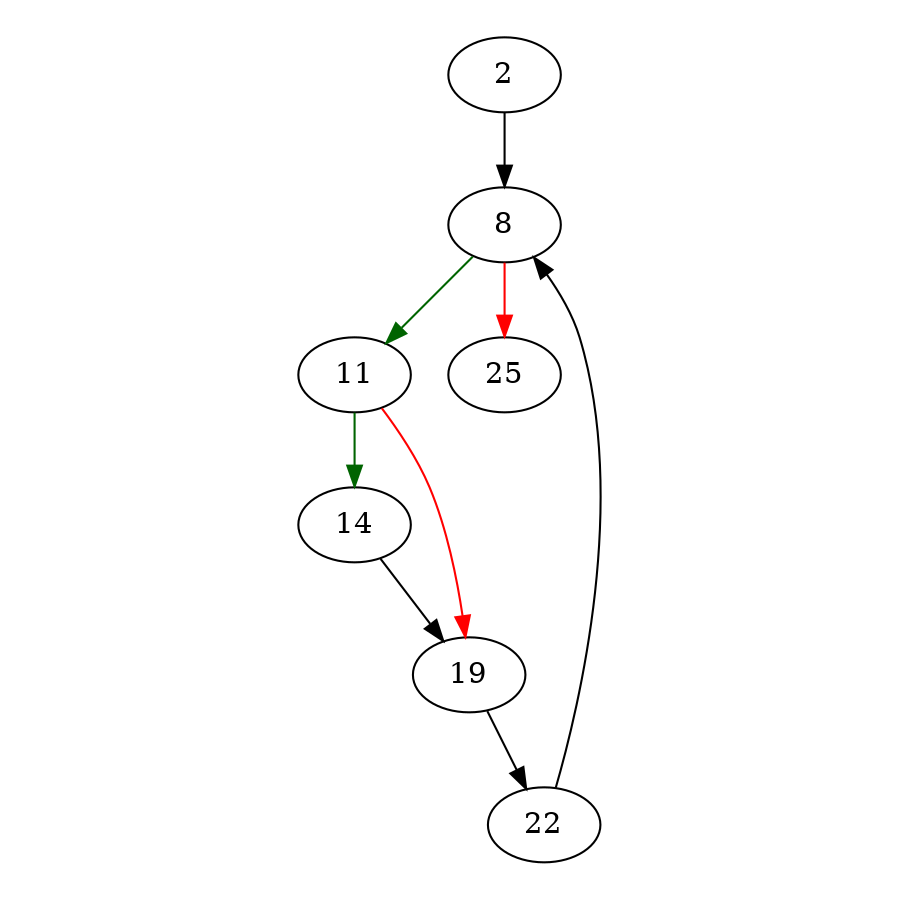
\includegraphics[width=\textwidth]{inc/appendices/examples/hammock/example/without-break/main.png}
		\caption{Control flow graph.}
	\end{subfigure}
\end{figure}

\begin{figure}[htbp]
	\centering
	\begin{subfigure}[b]{0.48\textwidth}
		\centering
		\lstinputlisting[linebackgroundcolor={\btLstHL{9-10}}, language=C, style=c, breaklines=false]{inc/appendices/examples/hammock/example/without-break.c}
		\caption{Original C source code.}
	\end{subfigure}
	\begin{subfigure}[b]{0.50\textwidth}
		\centering
		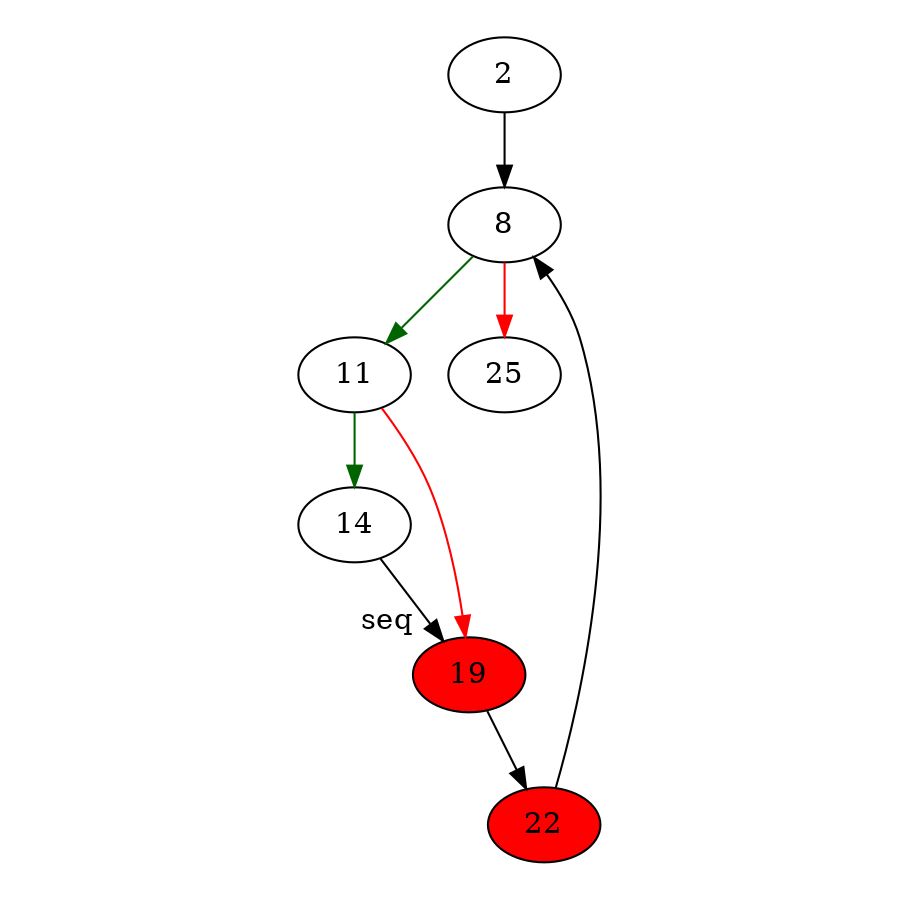
\includegraphics[width=\textwidth]{inc/appendices/examples/hammock/example/without-break/main_0001a.png}
		\caption{Control flow graph.}
	\end{subfigure}
\end{figure}

\begin{figure}[htbp]
	\centering
	\begin{subfigure}[b]{0.48\textwidth}
		\centering
		\lstinputlisting[linebackgroundcolor={\btLstHL{9-10}}, language=C, style=c, breaklines=false]{inc/appendices/examples/hammock/example/without-break.c}
		\caption{Original C source code.}
	\end{subfigure}
	\begin{subfigure}[b]{0.50\textwidth}
		\centering
		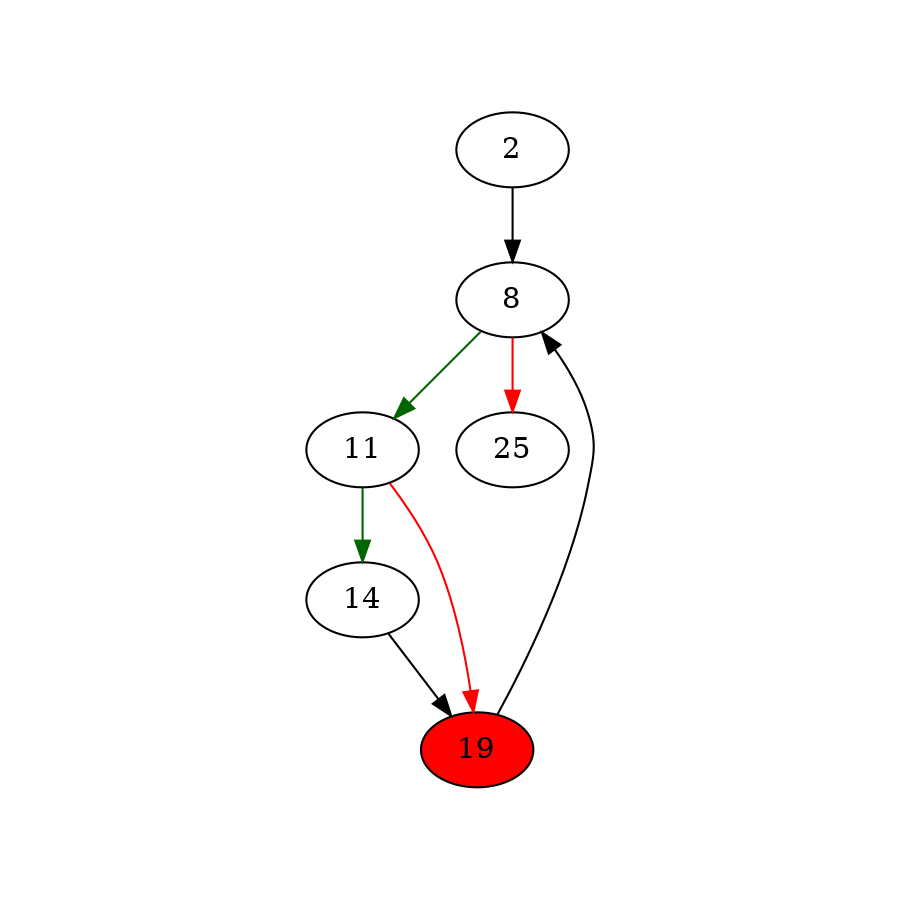
\includegraphics[width=\textwidth]{inc/appendices/examples/hammock/example/without-break/main_0001b.png}
		\caption{Control flow graph.}
	\end{subfigure}
\end{figure}

\begin{figure}[htbp]
	\centering
	\begin{subfigure}[b]{0.48\textwidth}
		\centering
		\lstinputlisting[linebackgroundcolor={\btLstHL{6-8}}, language=C, style=c, breaklines=false]{inc/appendices/examples/hammock/example/without-break.c}
		\caption{Original C source code.}
	\end{subfigure}
	\begin{subfigure}[b]{0.50\textwidth}
		\centering
		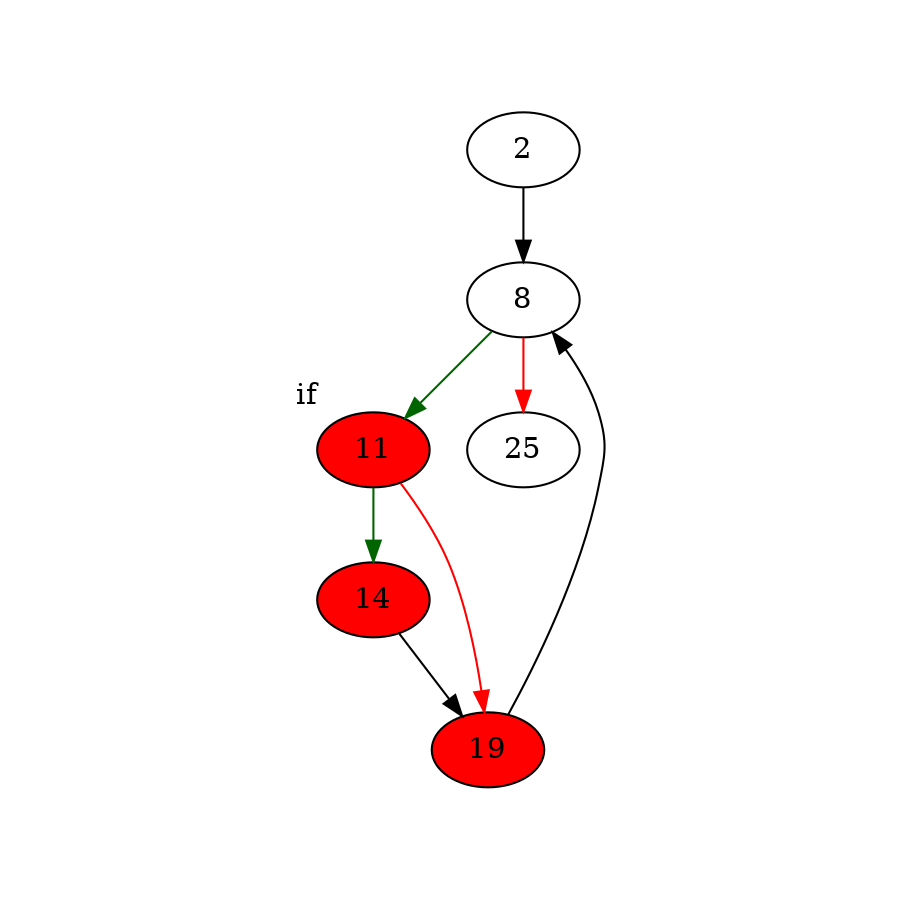
\includegraphics[width=\textwidth]{inc/appendices/examples/hammock/example/without-break/main_0002a.png}
		\caption{Control flow graph.}
	\end{subfigure}
\end{figure}

\begin{figure}[htbp]
	\centering
	\begin{subfigure}[b]{0.48\textwidth}
		\centering
		\lstinputlisting[linebackgroundcolor={\btLstHL{6-8}}, language=C, style=c, breaklines=false]{inc/appendices/examples/hammock/example/without-break.c}
		\caption{Original C source code.}
	\end{subfigure}
	\begin{subfigure}[b]{0.50\textwidth}
		\centering
		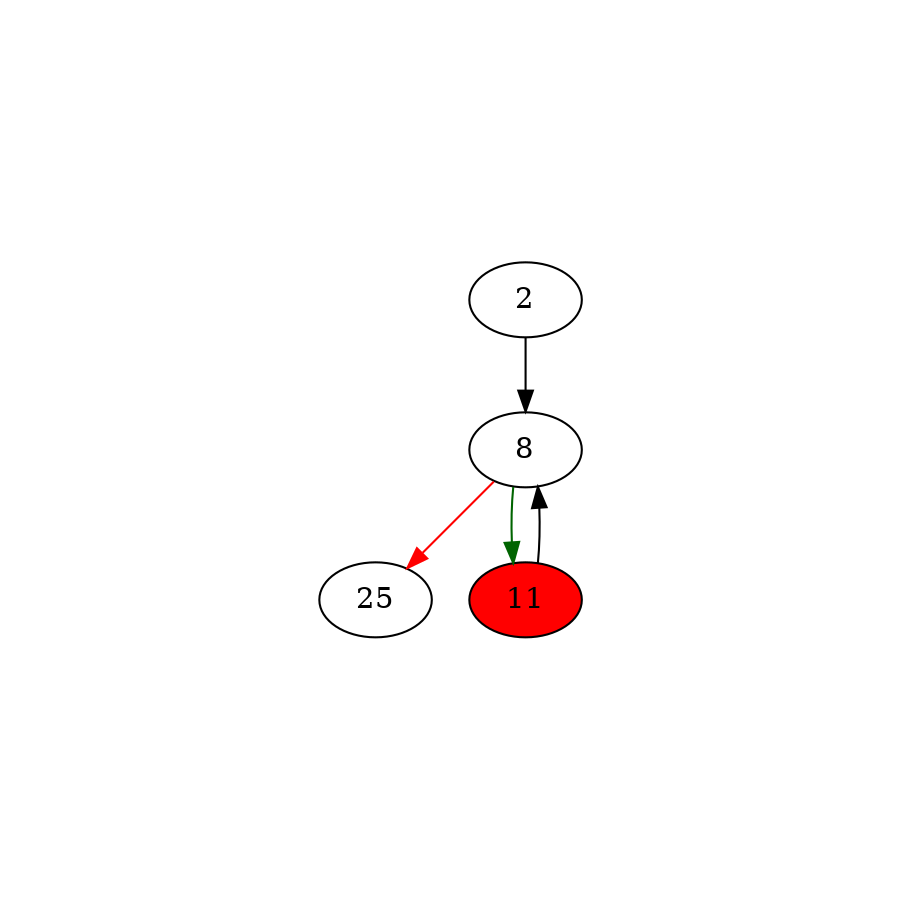
\includegraphics[width=\textwidth]{inc/appendices/examples/hammock/example/without-break/main_0002b.png}
		\caption{Control flow graph.}
	\end{subfigure}
\end{figure}

\begin{figure}[htbp]
	\centering
	\begin{subfigure}[b]{0.48\textwidth}
		\centering
		\lstinputlisting[linebackgroundcolor={\btLstHL{5, 10}}, language=C, style=c, breaklines=false]{inc/appendices/examples/hammock/example/without-break.c}
		\caption{Original C source code.}
	\end{subfigure}
	\begin{subfigure}[b]{0.50\textwidth}
		\centering
		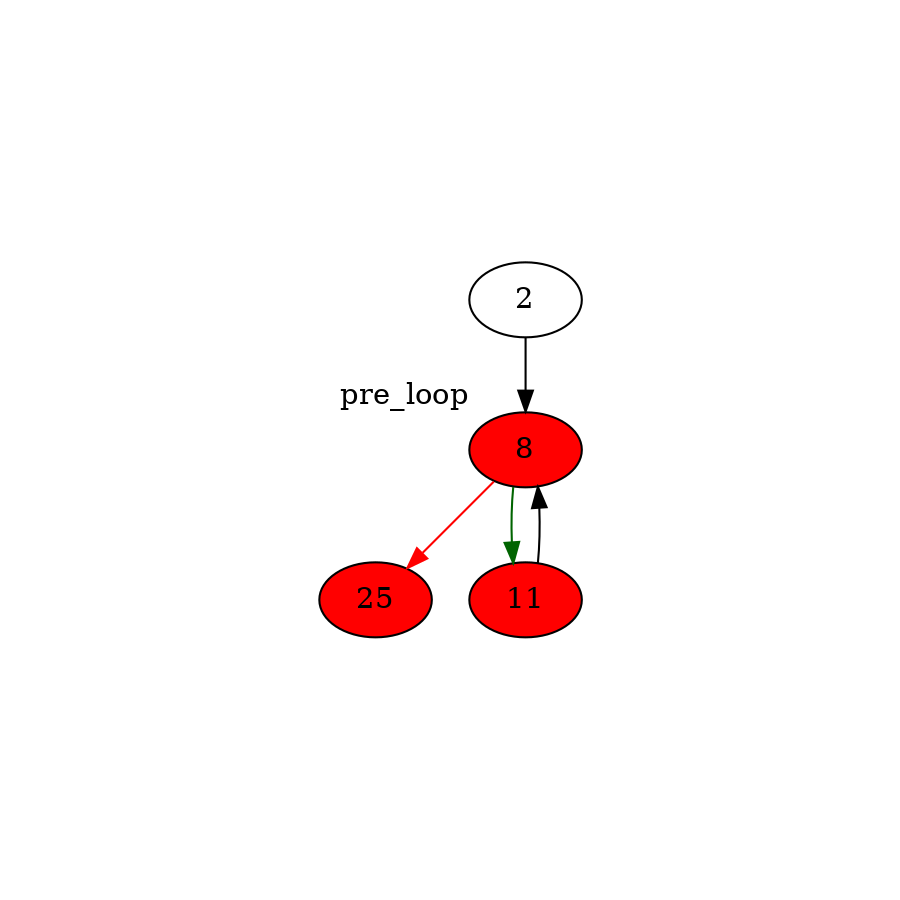
\includegraphics[width=\textwidth]{inc/appendices/examples/hammock/example/without-break/main_0003a.png}
		\caption{Control flow graph.}
	\end{subfigure}
\end{figure}

\begin{figure}[htbp]
	\centering
	\begin{subfigure}[b]{0.48\textwidth}
		\centering
		\lstinputlisting[linebackgroundcolor={\btLstHL{5, 10}}, language=C, style=c, breaklines=false]{inc/appendices/examples/hammock/example/without-break.c}
		\caption{Original C source code.}
	\end{subfigure}
	\begin{subfigure}[b]{0.50\textwidth}
		\centering
		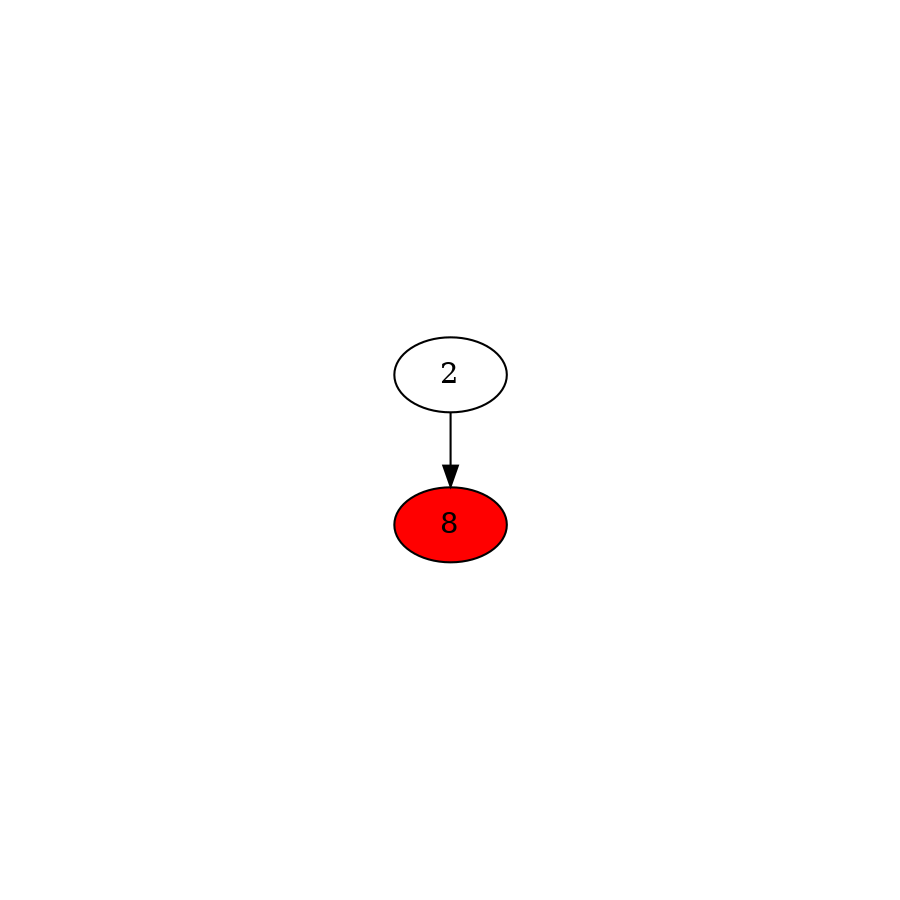
\includegraphics[width=\textwidth]{inc/appendices/examples/hammock/example/without-break/main_0003b.png}
		\caption{Control flow graph.}
	\end{subfigure}
\end{figure}

\begin{figure}[htbp]
	\centering
	\begin{subfigure}[b]{0.48\textwidth}
		\centering
		\lstinputlisting[linebackgroundcolor={\btLstHL{2-4}}, language=C, style=c, breaklines=false]{inc/appendices/examples/hammock/example/without-break.c}
		\caption{Original C source code.}
	\end{subfigure}
	\begin{subfigure}[b]{0.50\textwidth}
		\centering
		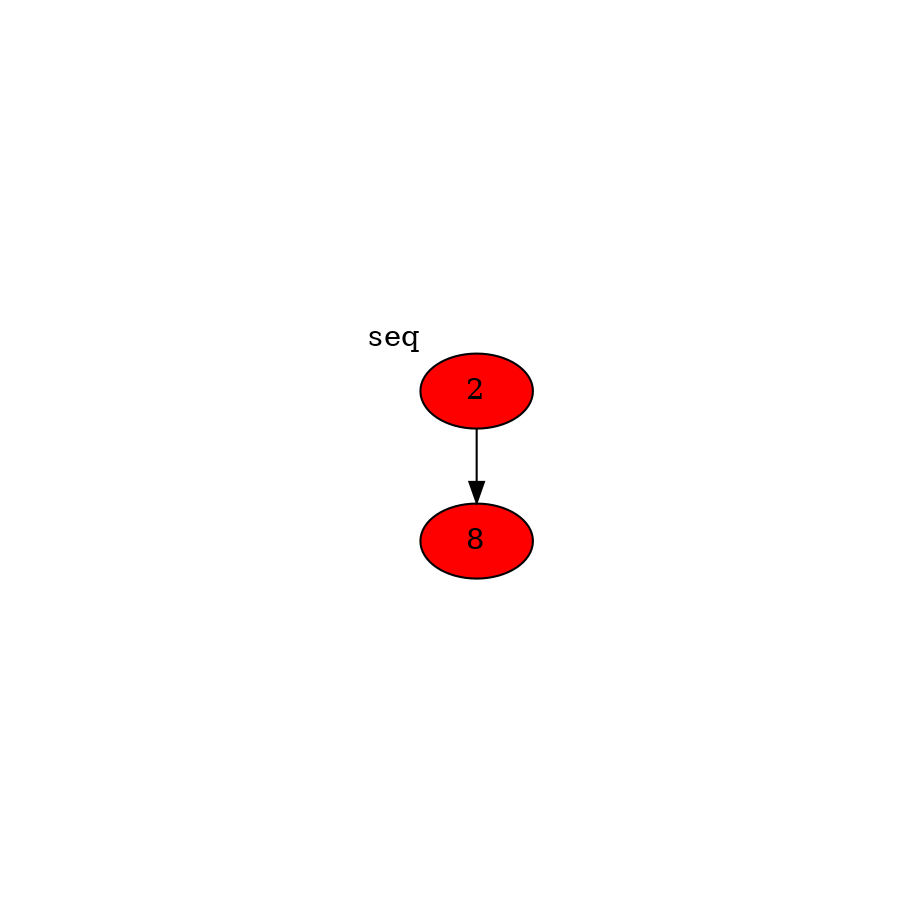
\includegraphics[width=\textwidth]{inc/appendices/examples/hammock/example/without-break/main_0004a.png}
		\caption{Control flow graph.}
	\end{subfigure}
\end{figure}

\begin{figure}[htbp]
	\centering
	\begin{subfigure}[b]{0.48\textwidth}
		\centering
		\lstinputlisting[linebackgroundcolor={\btLstHL{2-4}}, language=C, style=c, breaklines=false]{inc/appendices/examples/hammock/example/without-break.c}
		\caption{Original C source code.}
	\end{subfigure}
	\begin{subfigure}[b]{0.50\textwidth}
		\centering
		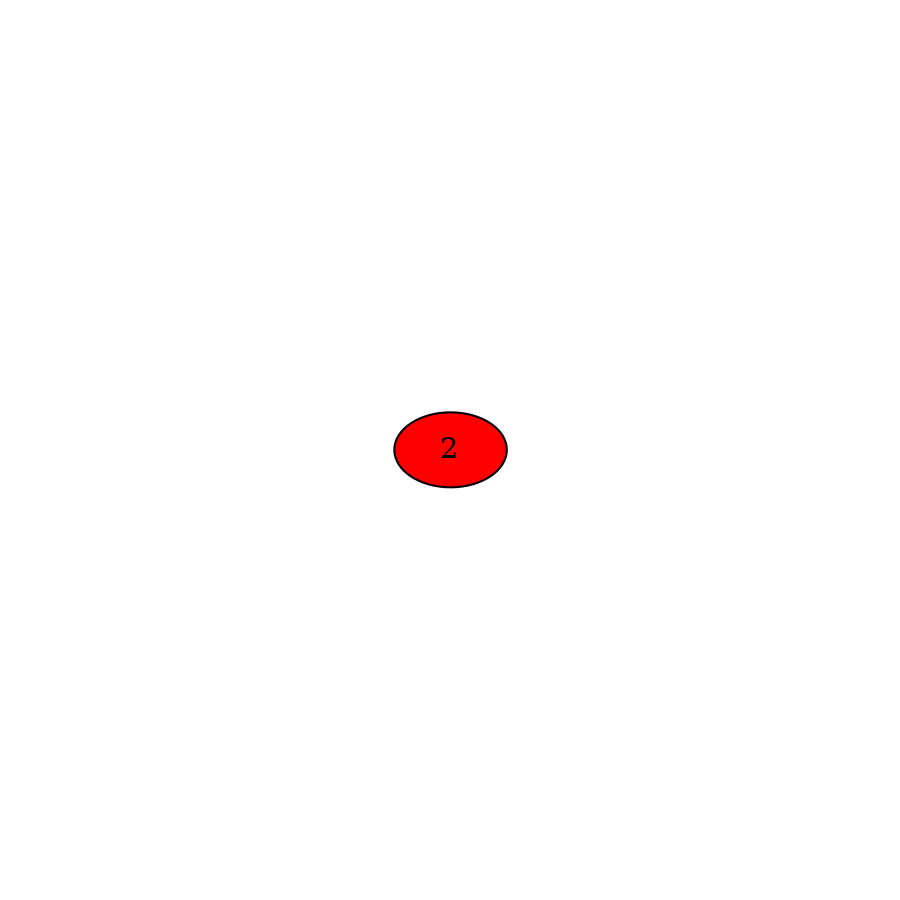
\includegraphics[width=\textwidth]{inc/appendices/examples/hammock/example/without-break/main_0004b.png}
		\caption{Control flow graph; analysis \textbf{complete}.}
	\end{subfigure}
\end{figure}

% ___ [ Hammock Method - Counter-example 1 ] ___________________________________

\clearpage

\subsubsection{Hammock Method - Counter-example 1}

Counter-example with \textit{multi-exit loop}.

\begin{figure}[htbp]
	\centering
	\begin{subfigure}[b]{0.48\textwidth}
		\centering
		\lstinputlisting[language=C, style=c, breaklines=false]{inc/appendices/examples/hammock/counter-example/with-break.c}
		\caption{Original C source code.}
	\end{subfigure}
	\begin{subfigure}[b]{0.50\textwidth}
		\centering
		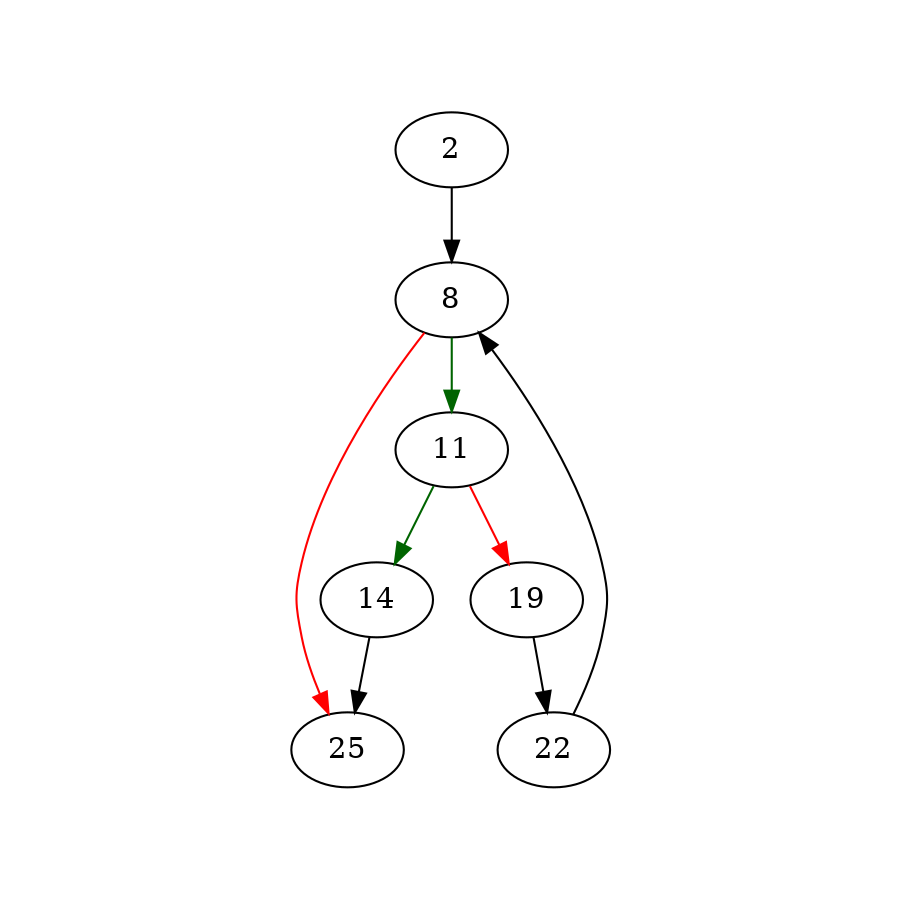
\includegraphics[width=\textwidth]{inc/appendices/examples/hammock/counter-example/with-break/main.png}
		\caption{Control flow graph.}
	\end{subfigure}
\end{figure}

\begin{figure}[htbp]
	\centering
	\begin{subfigure}[b]{0.48\textwidth}
		\centering
		\lstinputlisting[linebackgroundcolor={\btLstHL{10-11}}, language=C, style=c, breaklines=false]{inc/appendices/examples/hammock/counter-example/with-break.c}
		\caption{Original C source code.}
	\end{subfigure}
	\begin{subfigure}[b]{0.50\textwidth}
		\centering
		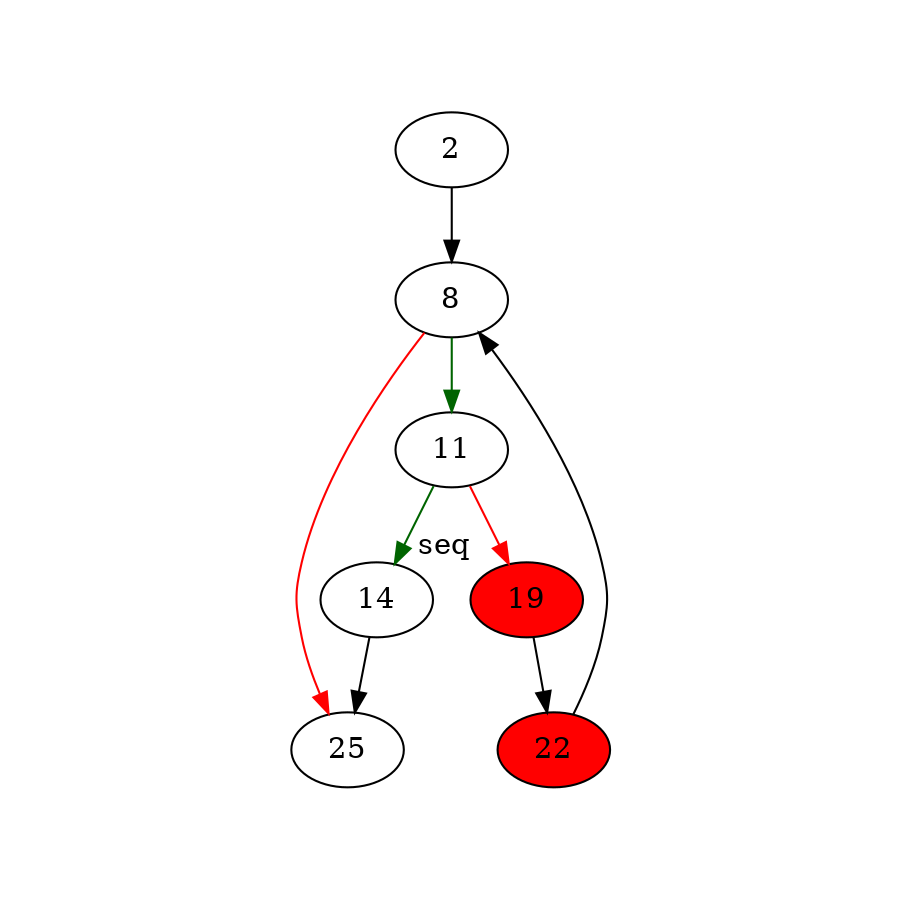
\includegraphics[width=\textwidth]{inc/appendices/examples/hammock/counter-example/with-break/main_0001a.png}
		\caption{Control flow graph.}
	\end{subfigure}
\end{figure}

\begin{figure}[htbp]
	\centering
	\begin{subfigure}[b]{0.48\textwidth}
		\centering
		\lstinputlisting[linebackgroundcolor={\btLstHL{10-11}}, language=C, style=c, breaklines=false]{inc/appendices/examples/hammock/counter-example/with-break.c}
		\caption{Original C source code.}
	\end{subfigure}
	\begin{subfigure}[b]{0.50\textwidth}
		\centering
		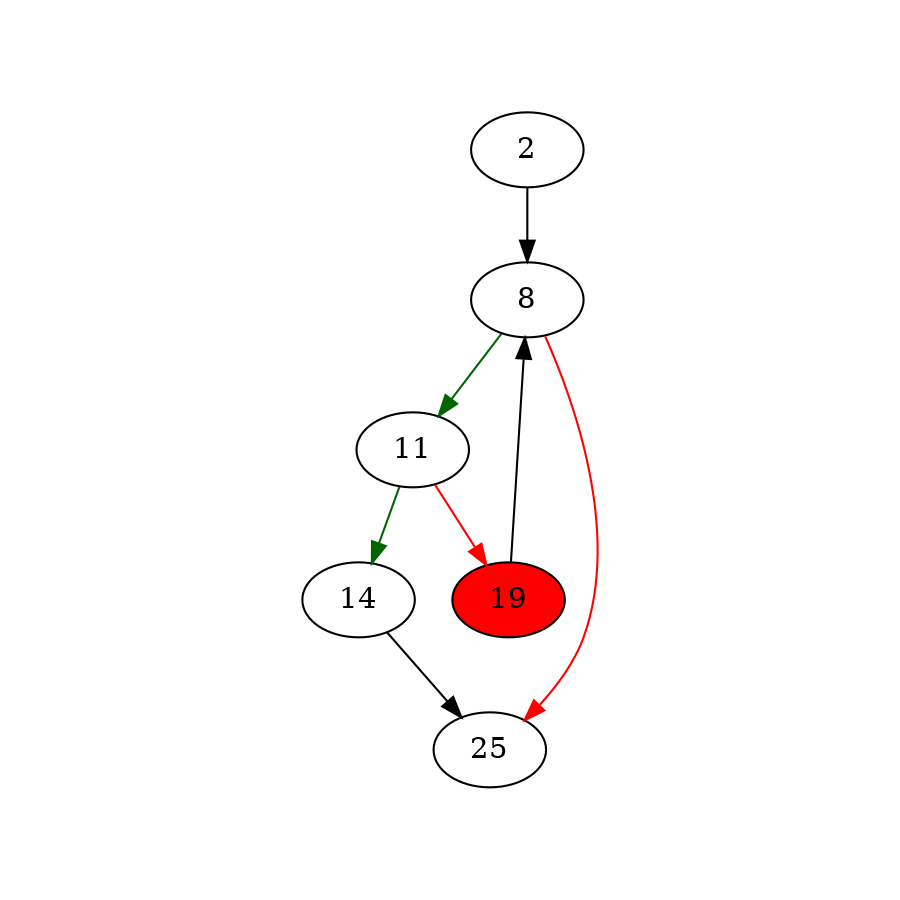
\includegraphics[width=\textwidth]{inc/appendices/examples/hammock/counter-example/with-break/main_0001b.png}
		\caption{Control flow graph; analysis \textbf{incomplete}.}
	\end{subfigure}
\end{figure}

% ___ [ Hammock Method - Counter-example 2 ] ___________________________________

\clearpage

\subsubsection{Hammock Method - Counter-example 2}

Counter-example with \textit{jump threading} optimization and \textit{short-circuit} evaluation.

\begin{figure}[htbp]
	\centering
	\begin{subfigure}[b]{0.30\textwidth}
		\centering
		\lstinputlisting[linerange={17-43}, language=C, style=c, breaklines=false]{inc/appendices/examples/hammock/counter-example/jump-threading-and-short-circuit/jump-threading-and-short-circuit.c}
		\caption{Original C source code.}
	\end{subfigure}
	\begin{subfigure}[b]{0.50\textwidth}
		\centering
		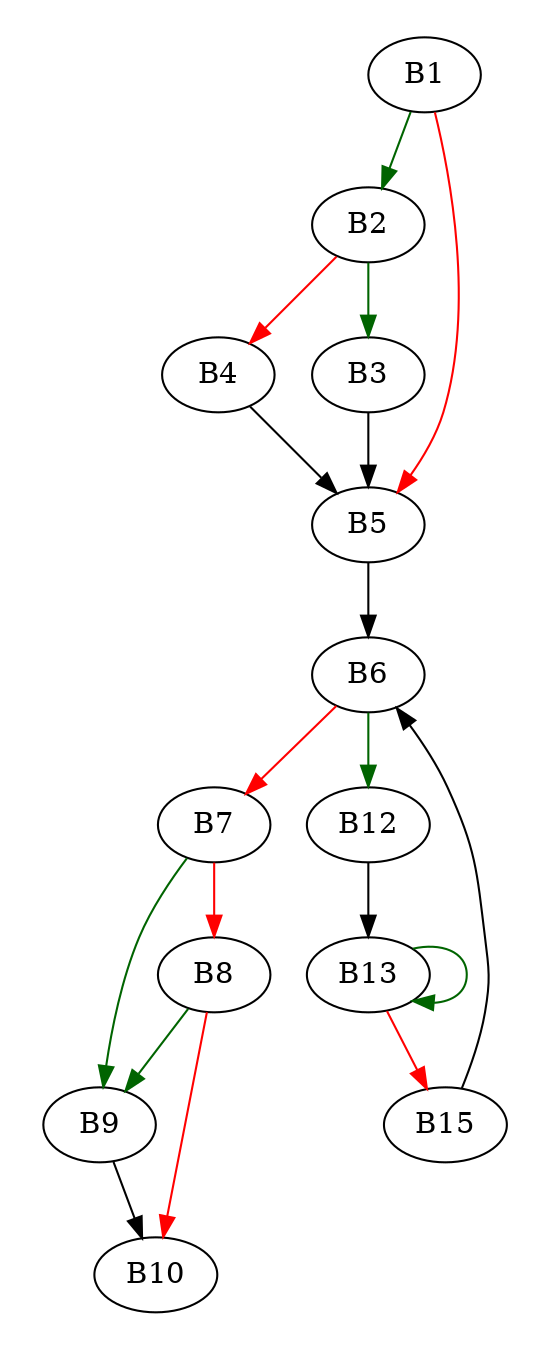
\includegraphics[width=0.6\textwidth]{inc/appendices/examples/hammock/counter-example/jump-threading-and-short-circuit/jump-threading-and-short-circuit_jump/f.png}
		\caption{Control flow graph.}
	\end{subfigure}
\end{figure}

\begin{figure}[htbp]
	\centering
	\begin{subfigure}[b]{0.30\textwidth}
		\centering
		\lstinputlisting[linebackgroundcolor={\btLstHL{15-18}}, linerange={17-43}, language=C, style=c, breaklines=false]{inc/appendices/examples/hammock/counter-example/jump-threading-and-short-circuit/jump-threading-and-short-circuit.c}
		\caption{Original C source code.}
	\end{subfigure}
	\begin{subfigure}[b]{0.50\textwidth}
		\centering
		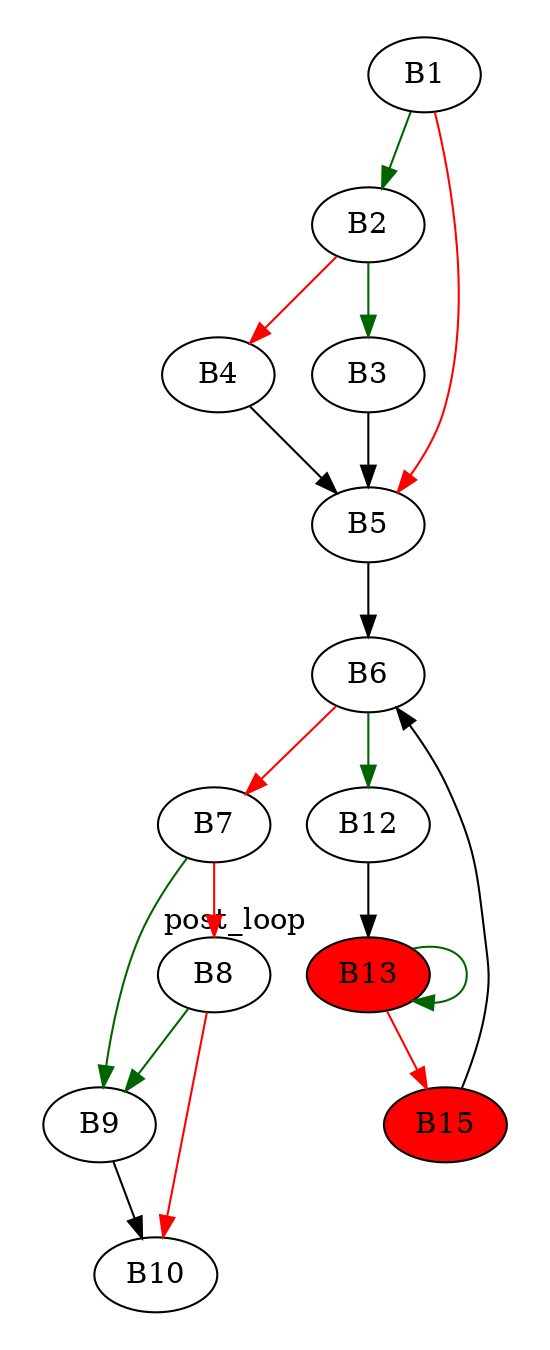
\includegraphics[width=0.6\textwidth]{inc/appendices/examples/hammock/counter-example/jump-threading-and-short-circuit/jump-threading-and-short-circuit_jump/f_0001a.png}
		\caption{Control flow graph.}
	\end{subfigure}
\end{figure}

\begin{figure}[htbp]
	\centering
	\begin{subfigure}[b]{0.30\textwidth}
		\centering
		\lstinputlisting[linebackgroundcolor={\btLstHL{15-18}}, linerange={17-43}, language=C, style=c, breaklines=false]{inc/appendices/examples/hammock/counter-example/jump-threading-and-short-circuit/jump-threading-and-short-circuit.c}
		\caption{Original C source code.}
	\end{subfigure}
	\begin{subfigure}[b]{0.50\textwidth}
		\centering
		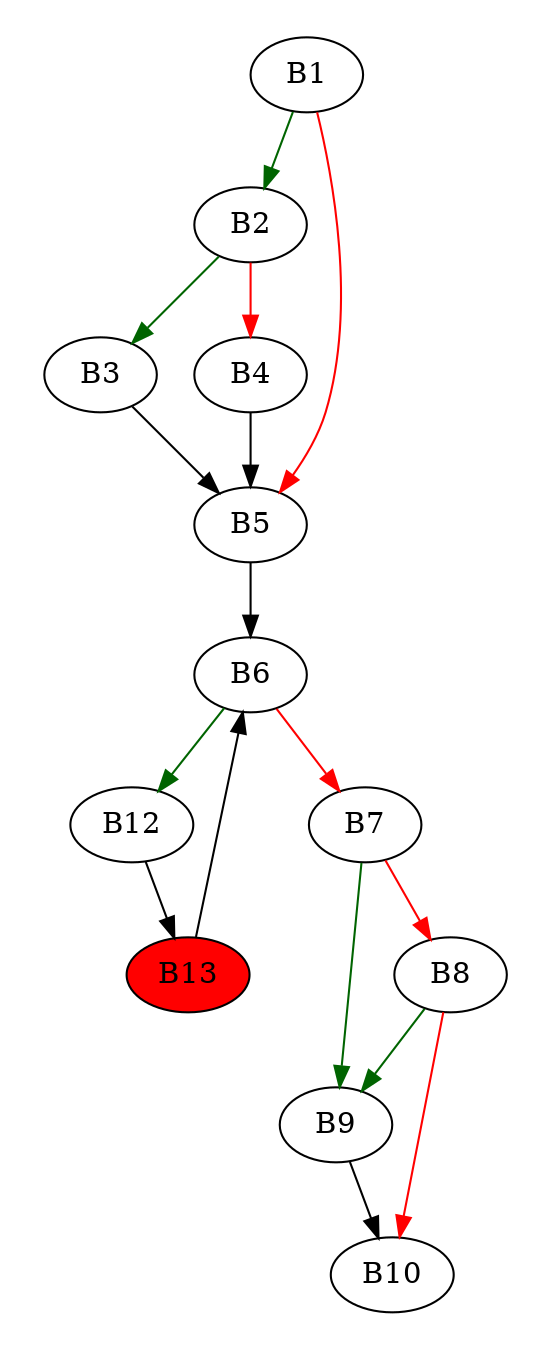
\includegraphics[width=0.6\textwidth]{inc/appendices/examples/hammock/counter-example/jump-threading-and-short-circuit/jump-threading-and-short-circuit_jump/f_0001b.png}
		\caption{Control flow graph.}
	\end{subfigure}
\end{figure}

\begin{figure}[htbp]
	\centering
	\begin{subfigure}[b]{0.30\textwidth}
		\centering
		\lstinputlisting[linebackgroundcolor={\btLstHL{13-14}}, linerange={17-43}, language=C, style=c, breaklines=false]{inc/appendices/examples/hammock/counter-example/jump-threading-and-short-circuit/jump-threading-and-short-circuit.c}
		\caption{Original C source code.}
	\end{subfigure}
	\begin{subfigure}[b]{0.50\textwidth}
		\centering
		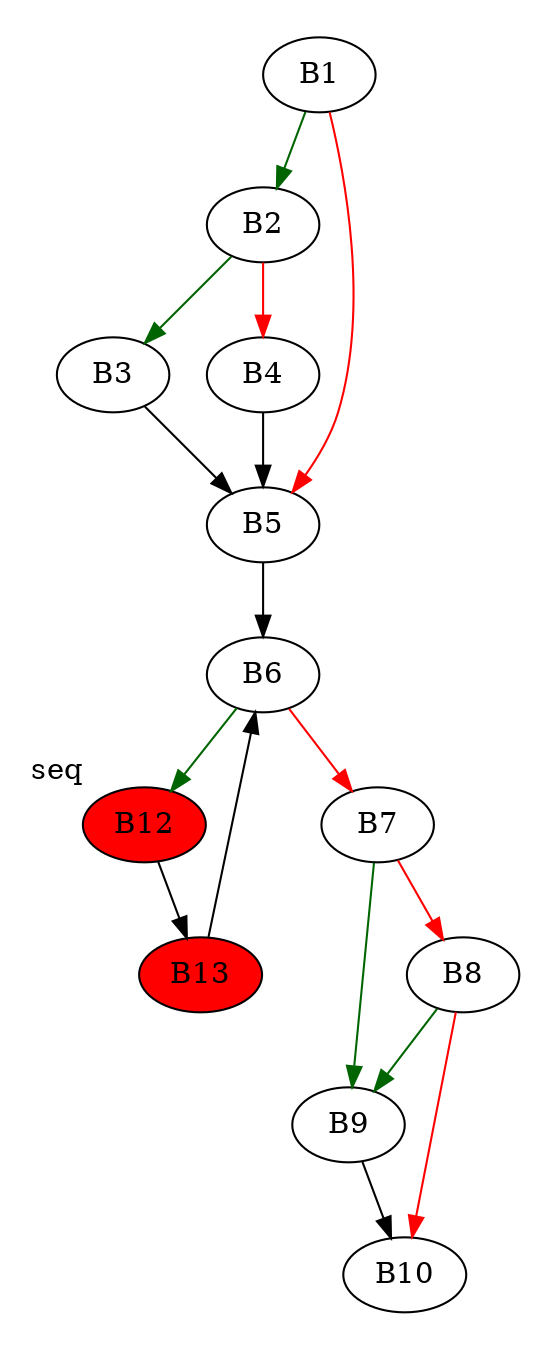
\includegraphics[width=0.6\textwidth]{inc/appendices/examples/hammock/counter-example/jump-threading-and-short-circuit/jump-threading-and-short-circuit_jump/f_0002a.png}
		\caption{Control flow graph.}
	\end{subfigure}
\end{figure}

\begin{figure}[htbp]
	\centering
	\begin{subfigure}[b]{0.30\textwidth}
		\centering
		\lstinputlisting[linebackgroundcolor={\btLstHL{13-14}}, linerange={17-43}, language=C, style=c, breaklines=false]{inc/appendices/examples/hammock/counter-example/jump-threading-and-short-circuit/jump-threading-and-short-circuit.c}
		\caption{Original C source code.}
	\end{subfigure}
	\begin{subfigure}[b]{0.50\textwidth}
		\centering
		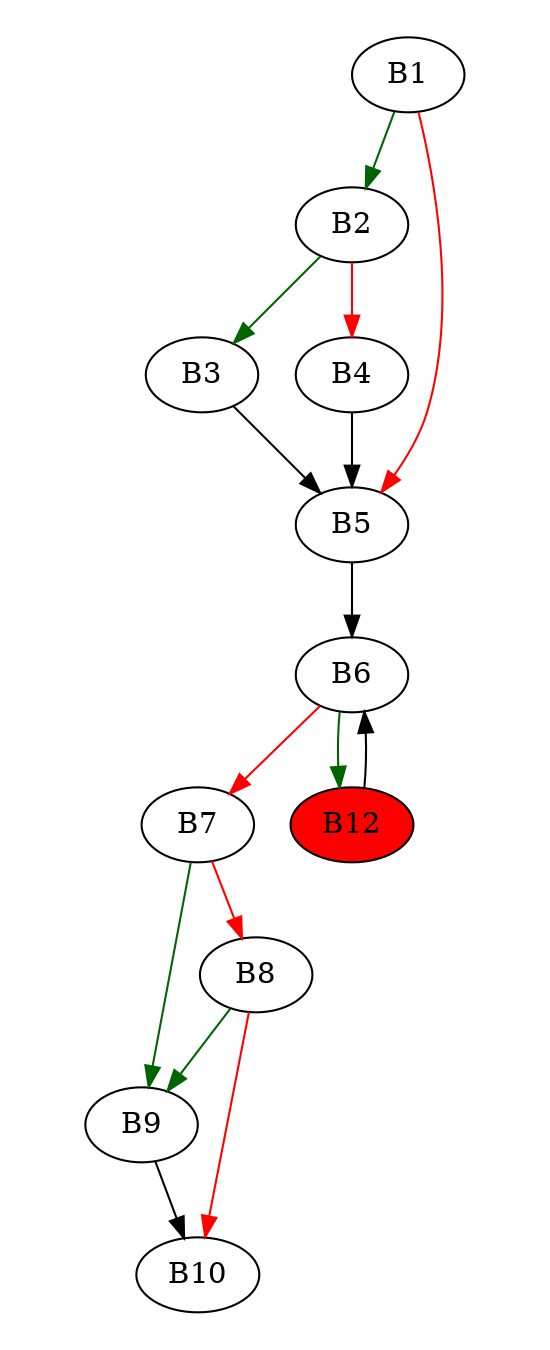
\includegraphics[width=0.6\textwidth]{inc/appendices/examples/hammock/counter-example/jump-threading-and-short-circuit/jump-threading-and-short-circuit_jump/f_0002b.png}
		\caption{Control flow graph.}
	\end{subfigure}
\end{figure}

\begin{figure}[htbp]
	\centering
	\begin{subfigure}[b]{0.30\textwidth}
		\centering
		\lstinputlisting[linebackgroundcolor={\btLstHL{12-13}}, linerange={17-43}, language=C, style=c, breaklines=false]{inc/appendices/examples/hammock/counter-example/jump-threading-and-short-circuit/jump-threading-and-short-circuit.c}
		\caption{Original C source code.}
	\end{subfigure}
	\begin{subfigure}[b]{0.50\textwidth}
		\centering
		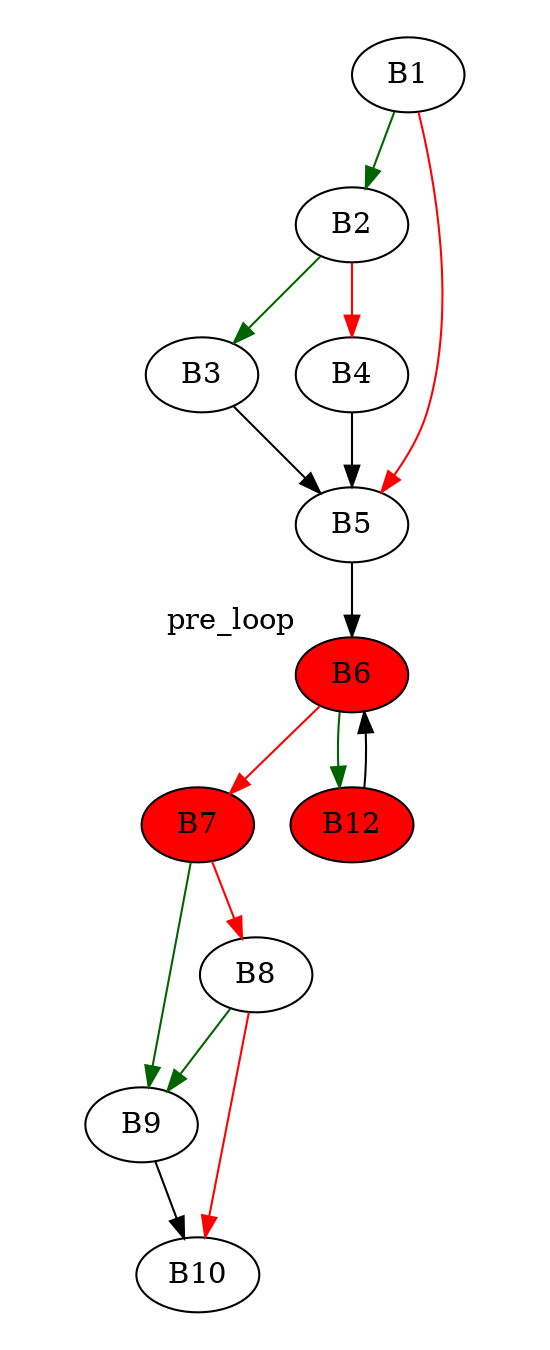
\includegraphics[width=0.6\textwidth]{inc/appendices/examples/hammock/counter-example/jump-threading-and-short-circuit/jump-threading-and-short-circuit_jump/f_0003a.png}
		\caption{Control flow graph.}
	\end{subfigure}
\end{figure}

\begin{figure}[htbp]
	\centering
	\begin{subfigure}[b]{0.30\textwidth}
		\centering
		\lstinputlisting[linebackgroundcolor={\btLstHL{12-13}}, linerange={17-43}, language=C, style=c, breaklines=false]{inc/appendices/examples/hammock/counter-example/jump-threading-and-short-circuit/jump-threading-and-short-circuit.c}
		\caption{Original C source code.}
	\end{subfigure}
	\begin{subfigure}[b]{0.50\textwidth}
		\centering
		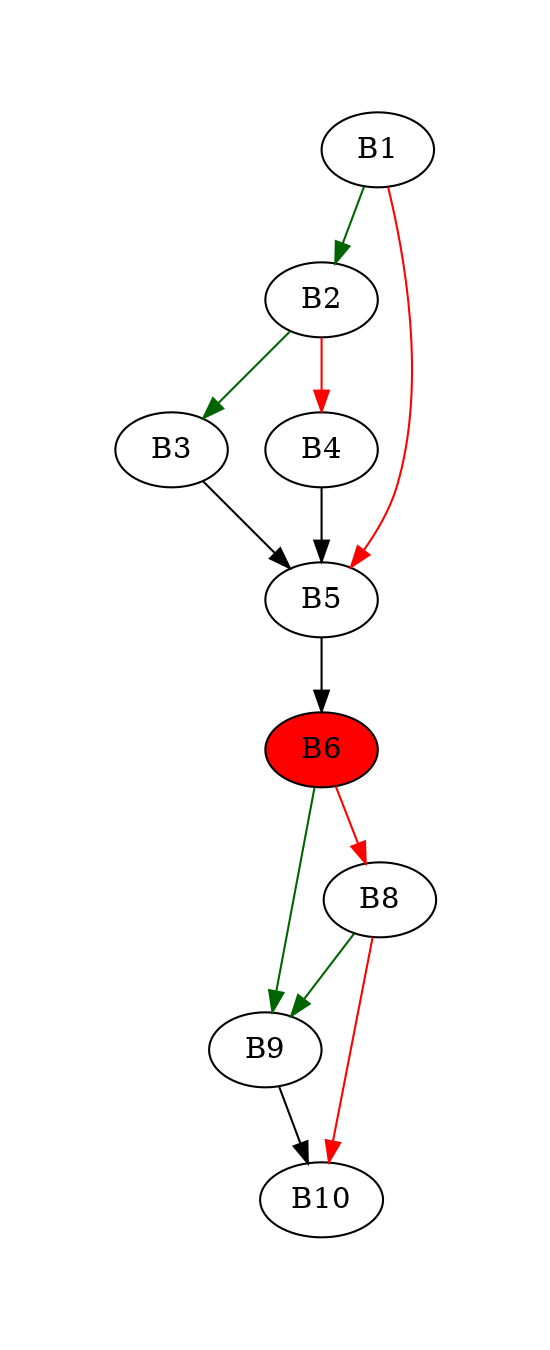
\includegraphics[width=0.6\textwidth]{inc/appendices/examples/hammock/counter-example/jump-threading-and-short-circuit/jump-threading-and-short-circuit_jump/f_0003b.png}
		\caption{Control flow graph.}
	\end{subfigure}
\end{figure}

\begin{figure}[htbp]
	\centering
	\begin{subfigure}[b]{0.30\textwidth}
		\centering
		\lstinputlisting[linebackgroundcolor={\btLstHL{11-12}}, linerange={17-43}, language=C, style=c, breaklines=false]{inc/appendices/examples/hammock/counter-example/jump-threading-and-short-circuit/jump-threading-and-short-circuit.c}
		\caption{Original C source code.}
	\end{subfigure}
	\begin{subfigure}[b]{0.50\textwidth}
		\centering
		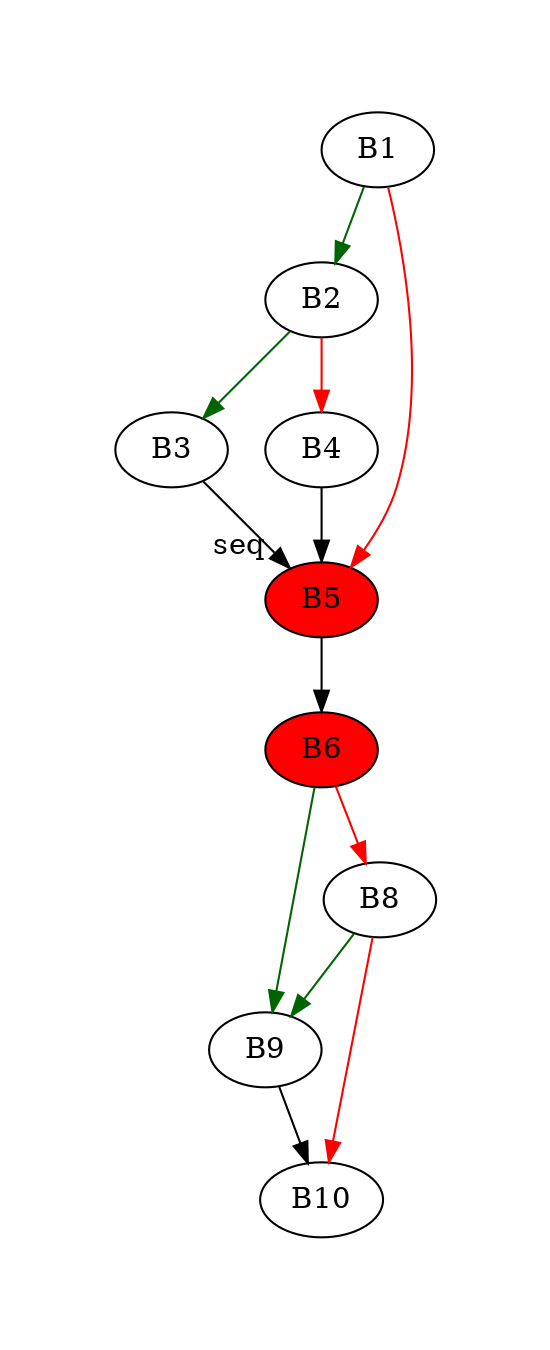
\includegraphics[width=0.6\textwidth]{inc/appendices/examples/hammock/counter-example/jump-threading-and-short-circuit/jump-threading-and-short-circuit_jump/f_0004a.png}
		\caption{Control flow graph.}
	\end{subfigure}
\end{figure}

\begin{figure}[htbp]
	\centering
	\begin{subfigure}[b]{0.30\textwidth}
		\centering
		\lstinputlisting[linebackgroundcolor={\btLstHL{11-12}}, linerange={17-43}, language=C, style=c, breaklines=false]{inc/appendices/examples/hammock/counter-example/jump-threading-and-short-circuit/jump-threading-and-short-circuit.c}
		\caption{Original C source code.}
	\end{subfigure}
	\begin{subfigure}[b]{0.50\textwidth}
		\centering
		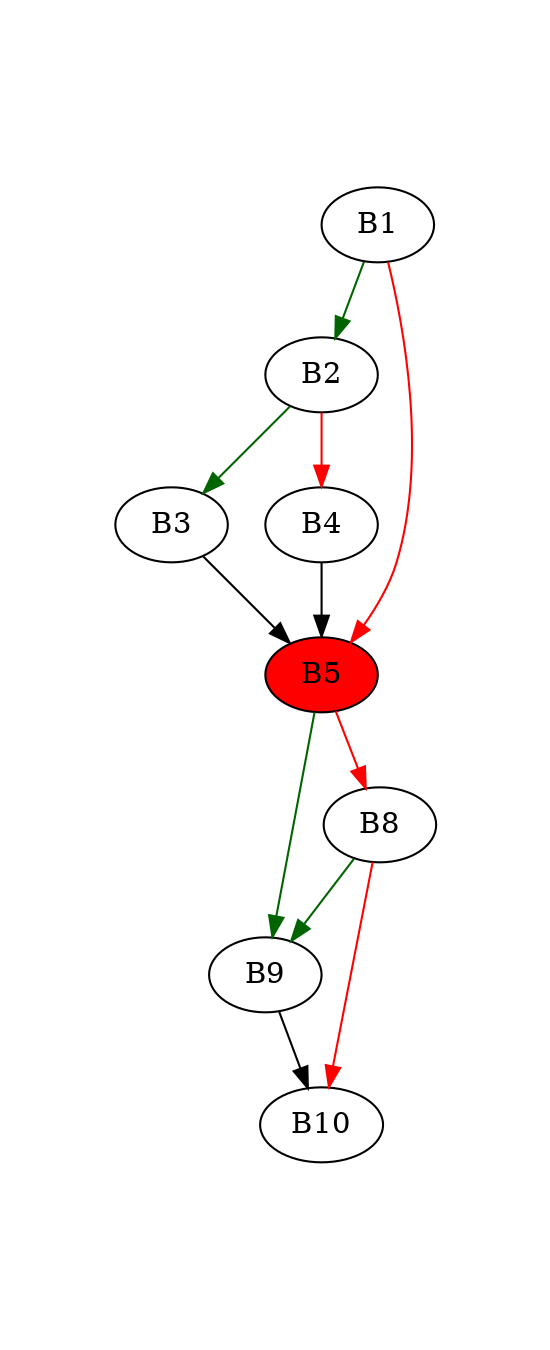
\includegraphics[width=0.6\textwidth]{inc/appendices/examples/hammock/counter-example/jump-threading-and-short-circuit/jump-threading-and-short-circuit_jump/f_0004b.png}
		\caption{Control flow graph; analysis \textbf{incomplete}.}
	\end{subfigure}
\end{figure}

% --- [ Interval method ] ------------------------------------------------------

% ___ [ Interval Method - Example 1 ] __________________________________________

\clearpage

\subsubsection{Interval Method - Example 1}

Example with \textit{jump threading} optimization and \textit{short-circuit} evaluation.

\begin{figure}[htbp]
	\centering
	\begin{subfigure}[b]{0.30\textwidth}
		\centering
		\lstinputlisting[linerange={17-43}, language=C, style=c, breaklines=false]{inc/appendices/examples/interval/example/sample.c}
		\caption{Original C source code.}
	\end{subfigure}
	\begin{subfigure}[b]{0.50\textwidth}
		\centering
		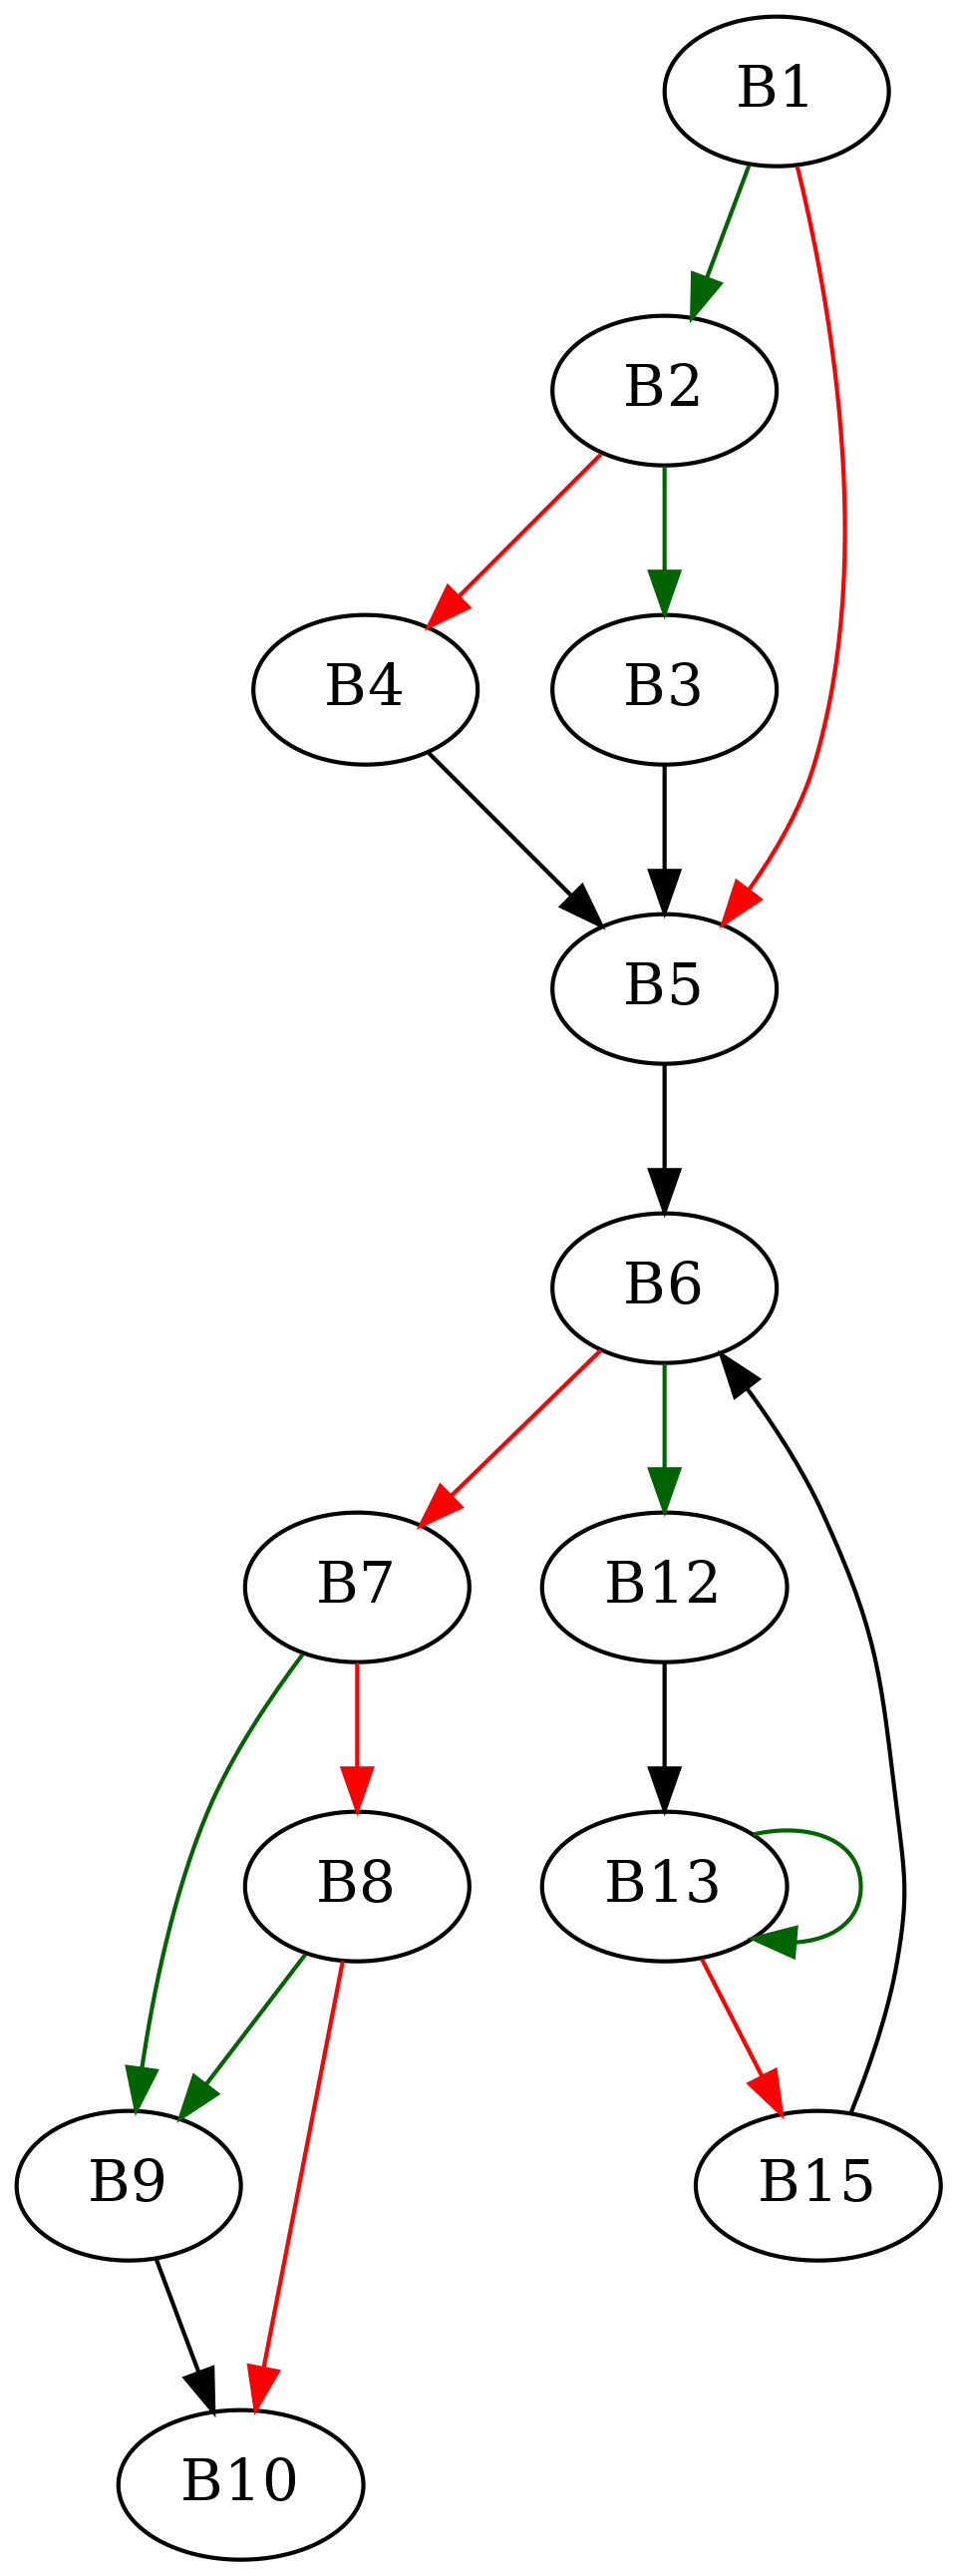
\includegraphics[width=0.6\textwidth]{inc/appendices/examples/interval/example/sample/f.png}
		\caption{Control flow graph.}
	\end{subfigure}
\end{figure}

\begin{figure}[htbp]
	\centering
	\begin{subfigure}[b]{0.30\textwidth}
		\centering
		\lstinputlisting[linerange={17-43}, linebackgroundcolor={\btLstHL{22}}, language=C, style=c, breaklines=false]{inc/appendices/examples/interval/example/sample.c}
		\caption{Original C source code.}
	\end{subfigure}
	\begin{subfigure}[b]{0.50\textwidth}
		\centering
		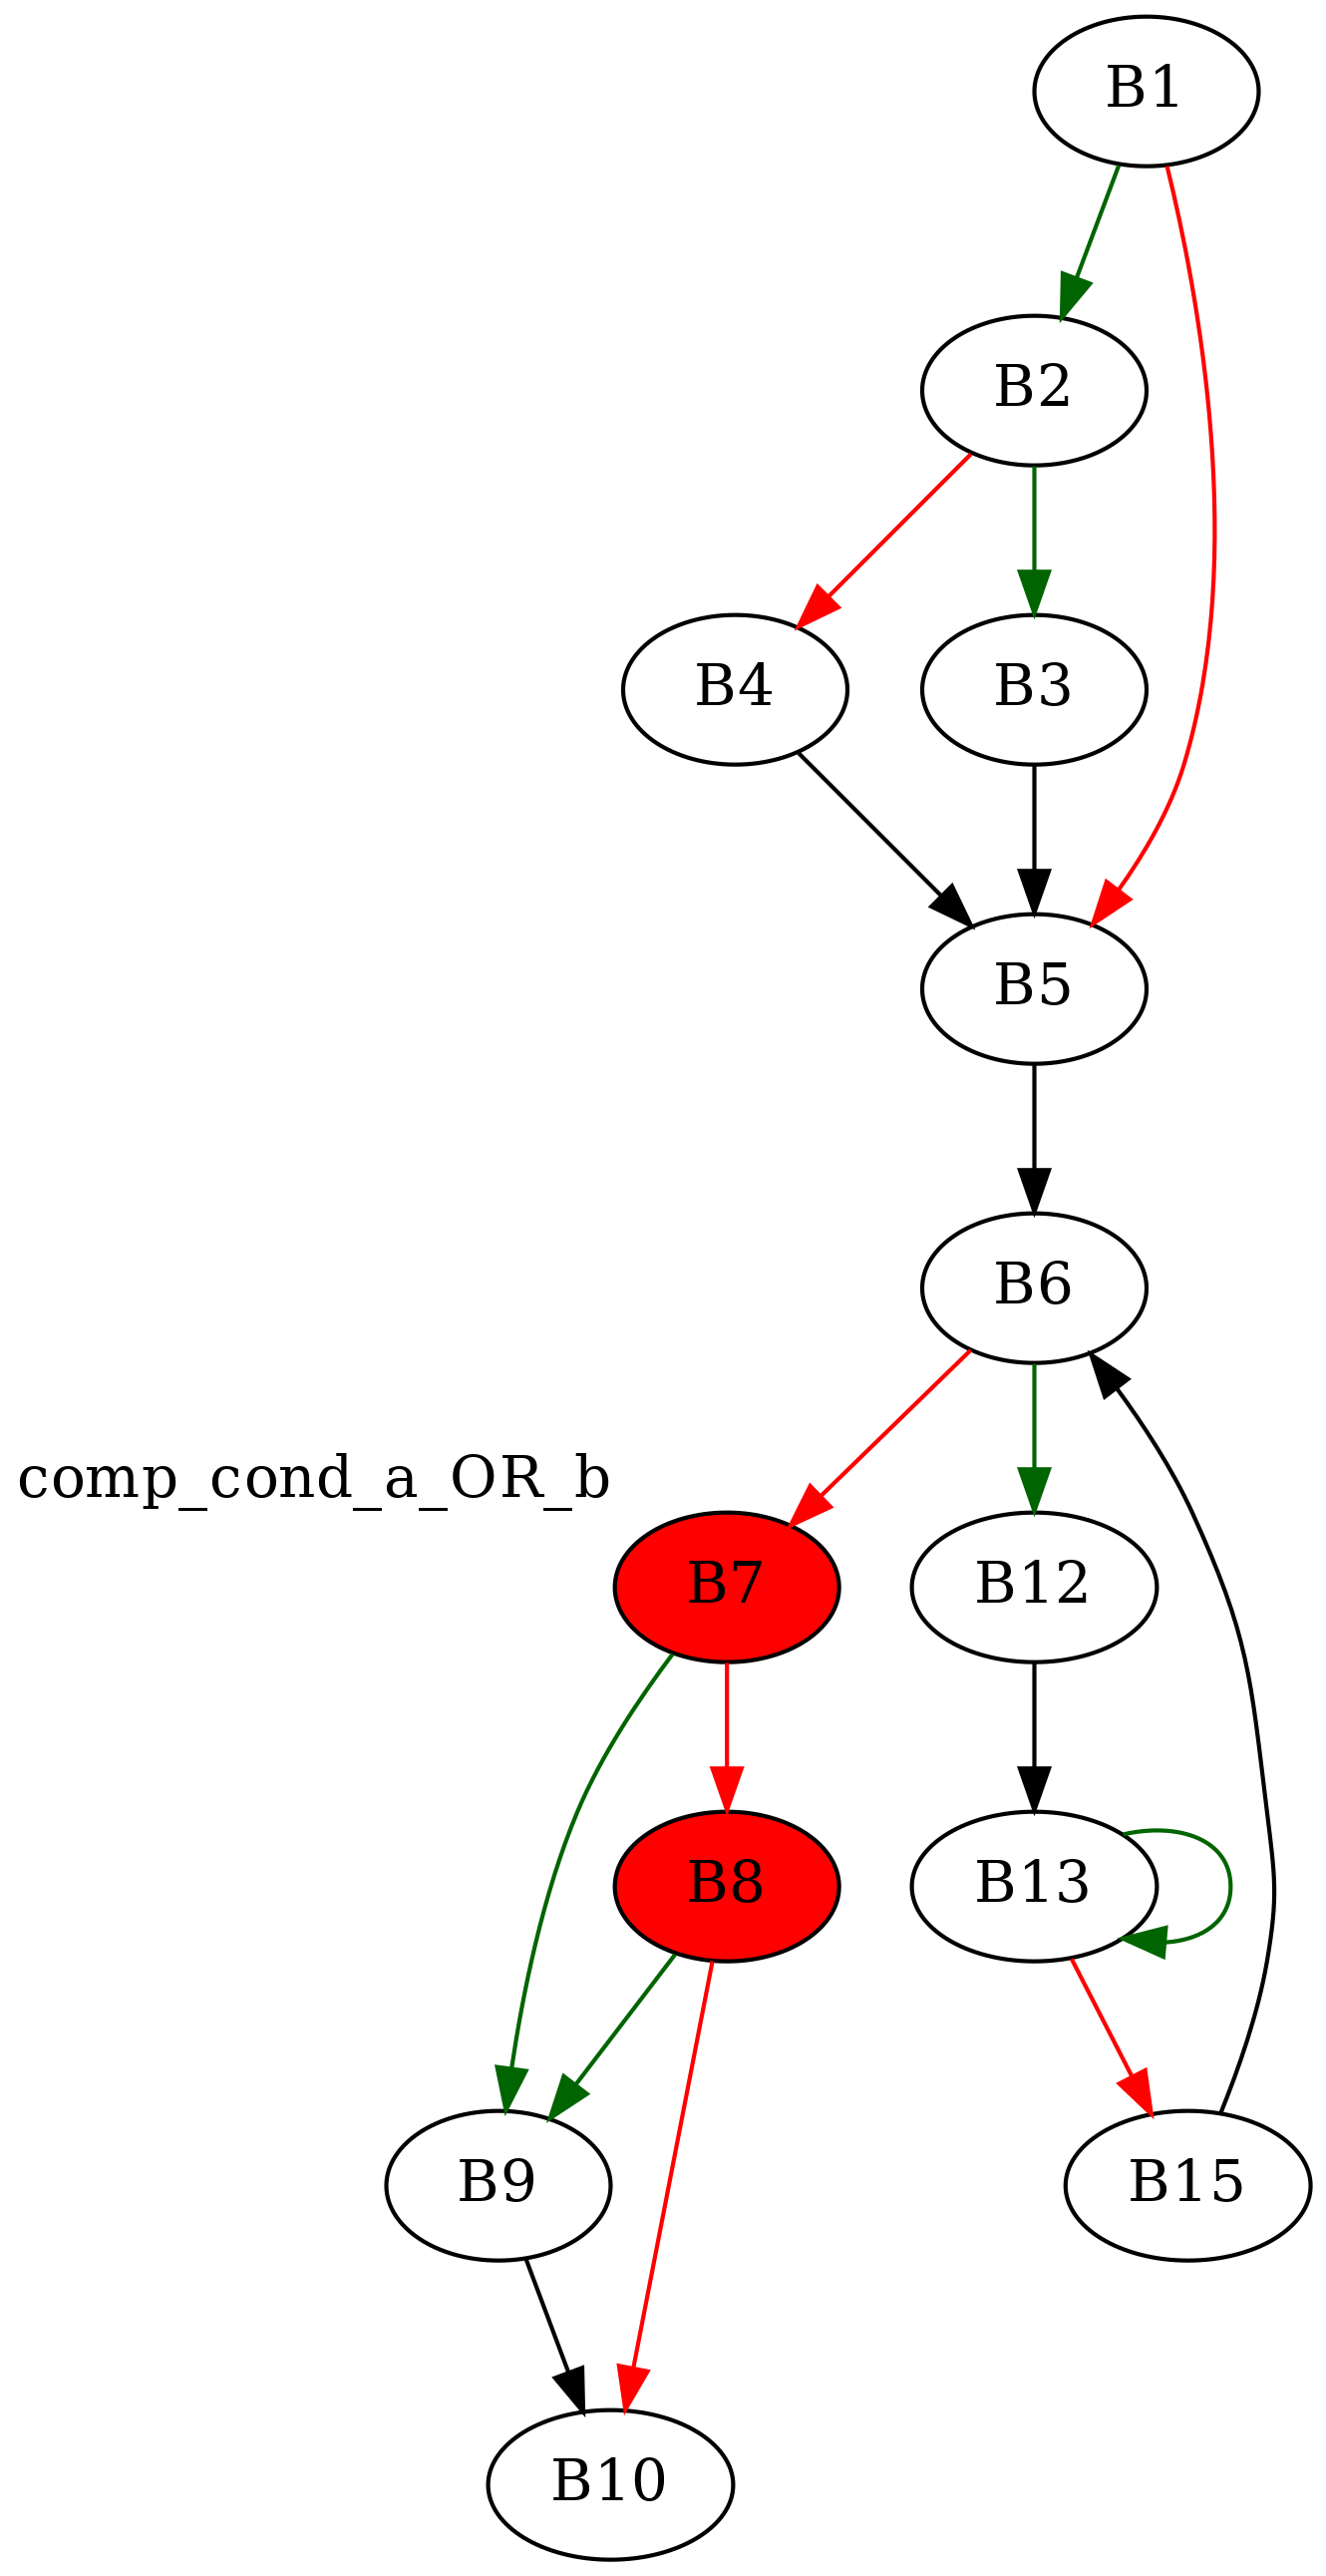
\includegraphics[width=0.8\textwidth]{inc/appendices/examples/interval/example/sample/f_0001a.png}
		\caption{Control flow graph.}
	\end{subfigure}
\end{figure}

\begin{figure}[htbp]
	\centering
	\begin{subfigure}[b]{0.30\textwidth}
		\centering
		\lstinputlisting[linerange={17-43}, linebackgroundcolor={\btLstHL{22}}, language=C, style=c, breaklines=false]{inc/appendices/examples/interval/example/sample.c}
		\caption{Original C source code.}
	\end{subfigure}
	\begin{subfigure}[b]{0.50\textwidth}
		\centering
		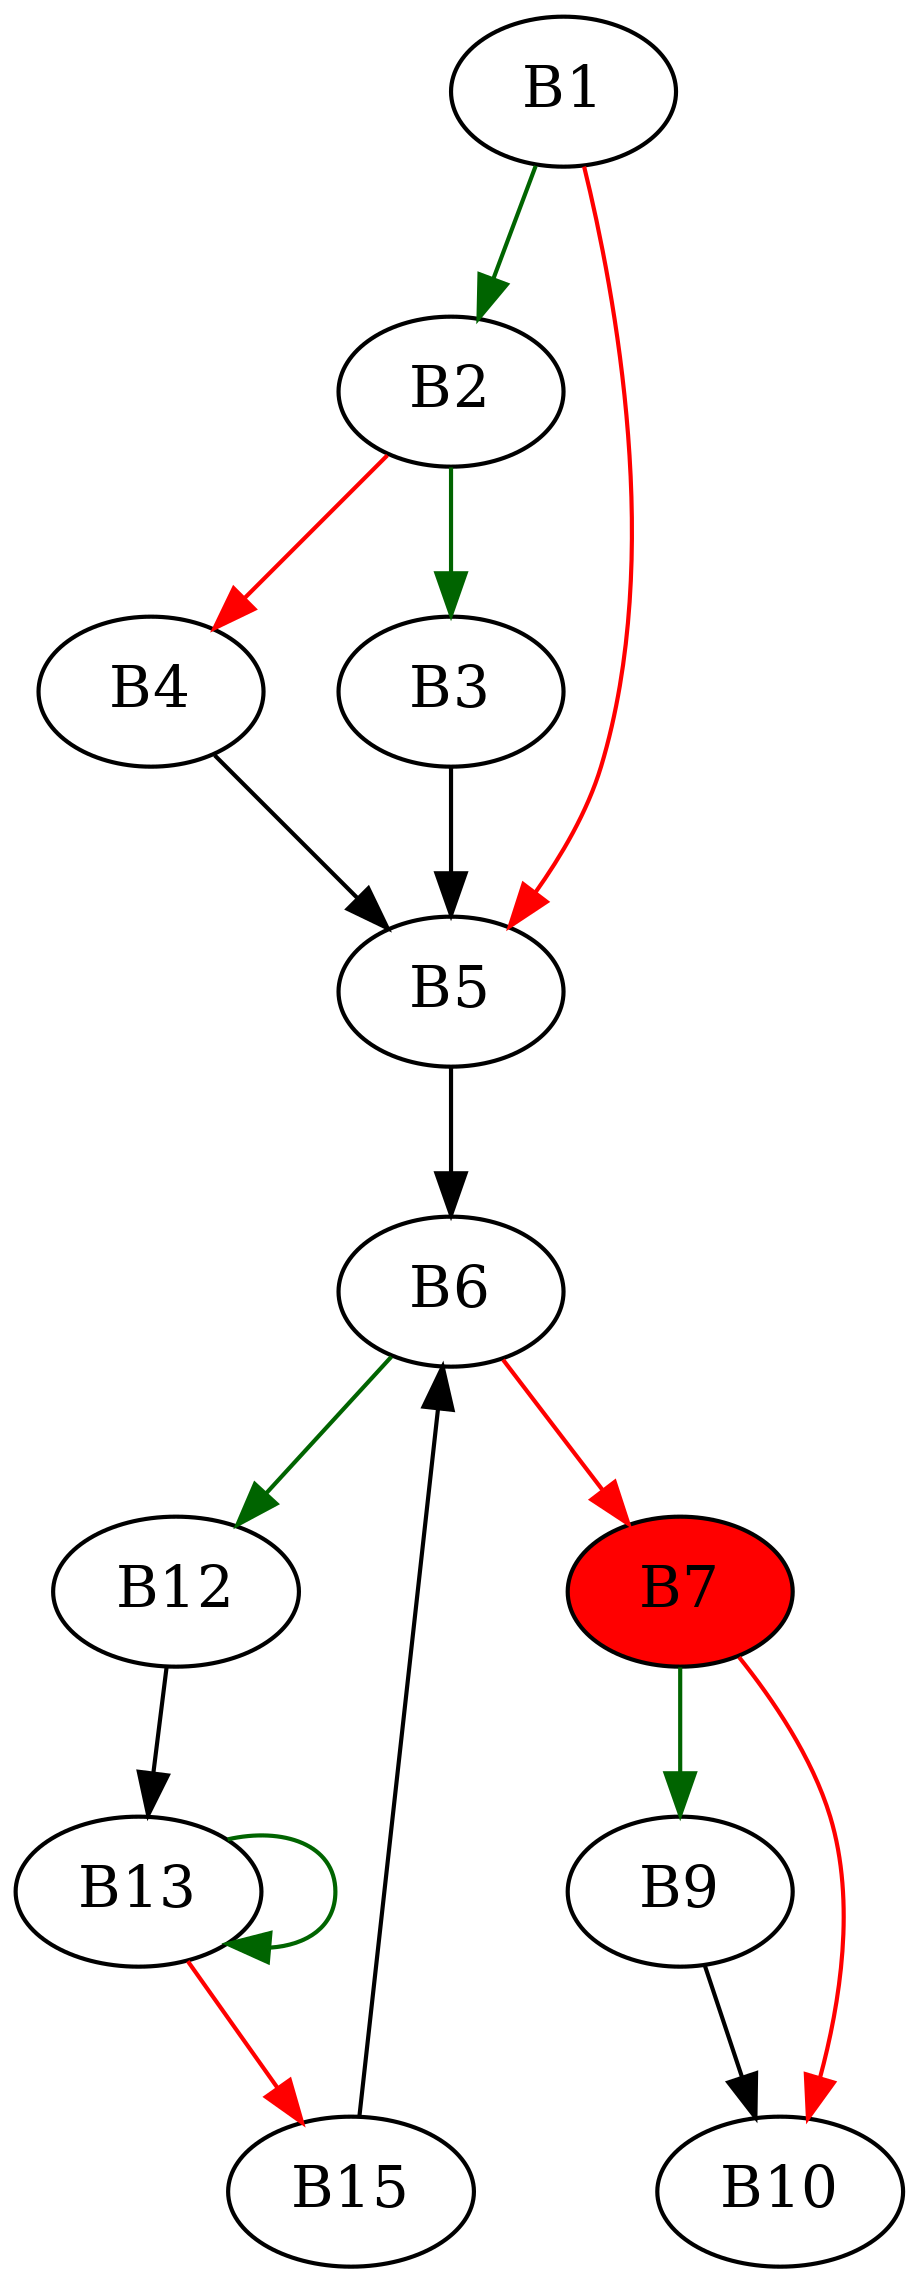
\includegraphics[width=0.6\textwidth]{inc/appendices/examples/interval/example/sample/f_0001b.png}
		\caption{Control flow graph.}
	\end{subfigure}
\end{figure}

\begin{figure}[htbp]
	\centering
	\begin{subfigure}[b]{0.30\textwidth}
		\centering
		\lstinputlisting[linerange={17-43}, linebackgroundcolor={\btLstHL{15-18}}, language=C, style=c, breaklines=false]{inc/appendices/examples/interval/example/sample.c}
		\caption{Original C source code.}
	\end{subfigure}
	\begin{subfigure}[b]{0.50\textwidth}
		\centering
		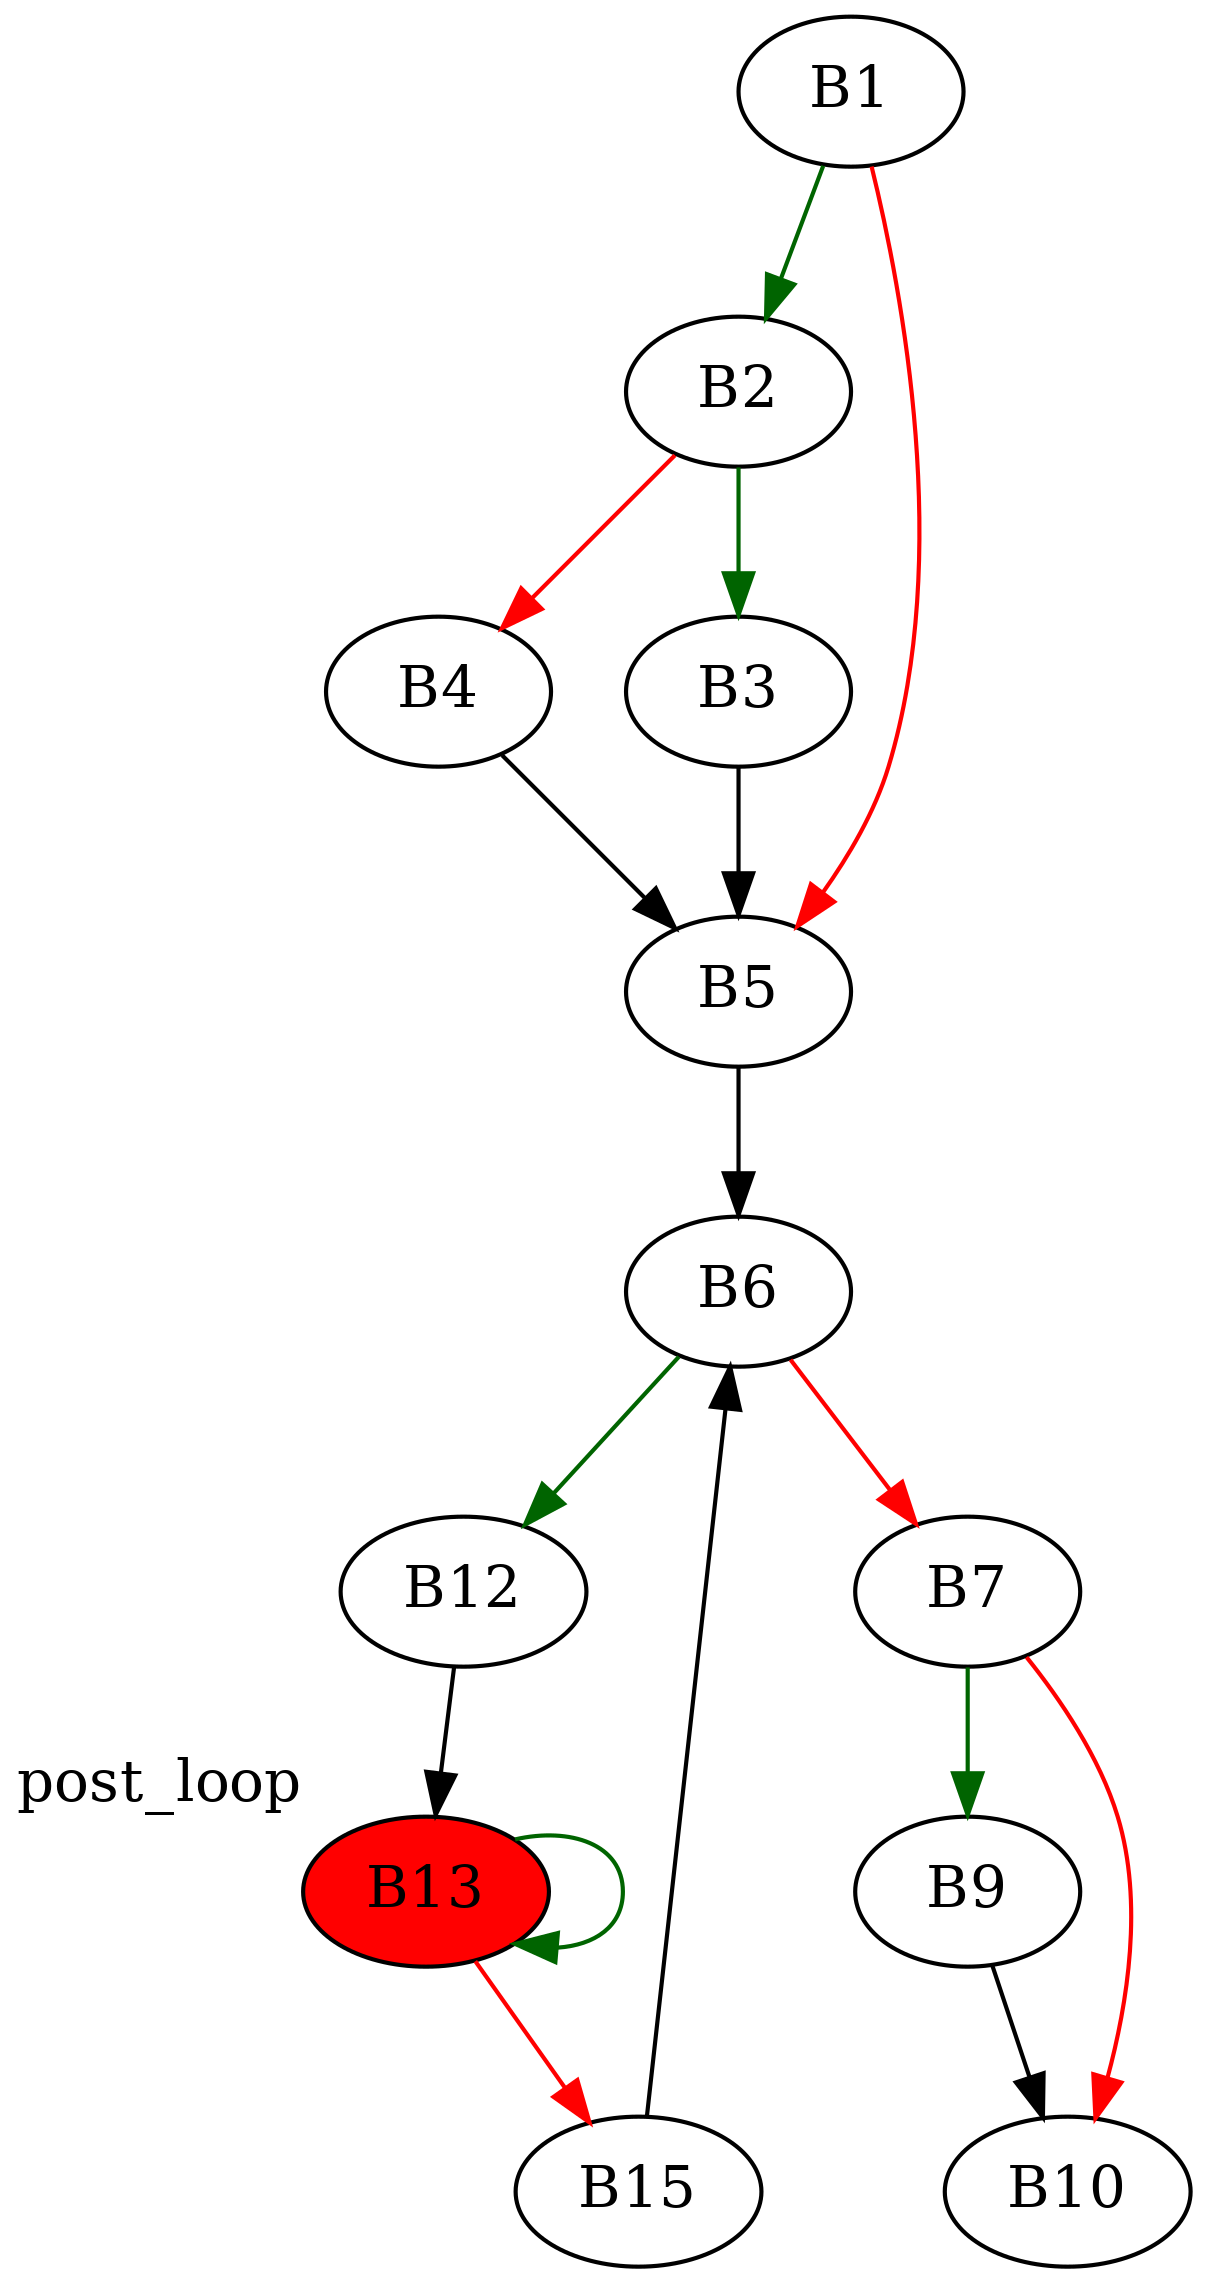
\includegraphics[width=0.75\textwidth]{inc/appendices/examples/interval/example/sample/f_0002a.png}
		\caption{Control flow graph.}
	\end{subfigure}
\end{figure}

\begin{figure}[htbp]
	\centering
	\begin{subfigure}[b]{0.30\textwidth}
		\centering
		\lstinputlisting[linerange={17-43}, linebackgroundcolor={\btLstHL{15-18}}, language=C, style=c, breaklines=false]{inc/appendices/examples/interval/example/sample.c}
		\caption{Original C source code.}
	\end{subfigure}
	\begin{subfigure}[b]{0.50\textwidth}
		\centering
		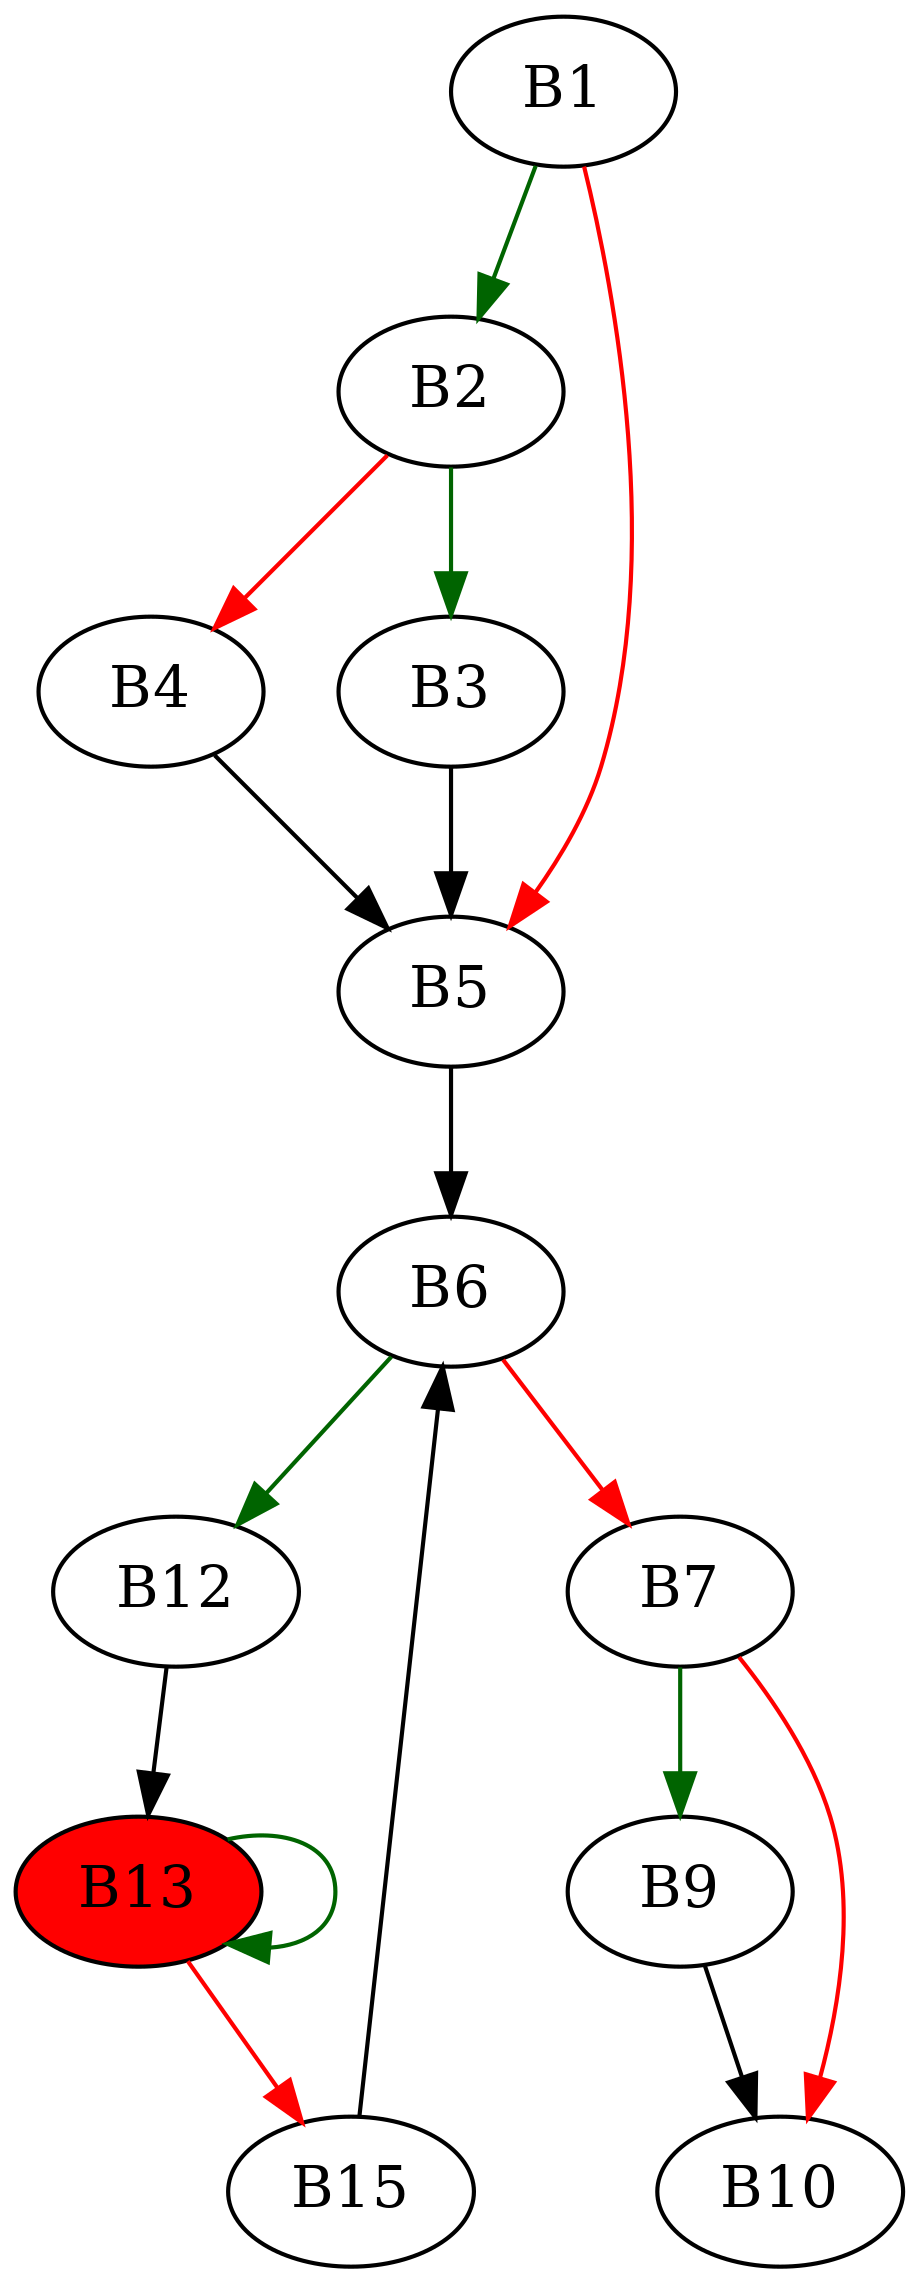
\includegraphics[width=0.6\textwidth]{inc/appendices/examples/interval/example/sample/f_0002b.png}
		\caption{Control flow graph.}
	\end{subfigure}
\end{figure}

\begin{figure}[htbp]
	\centering
	\begin{subfigure}[b]{0.30\textwidth}
		\centering
		\lstinputlisting[linerange={17-43}, linebackgroundcolor={\btLstHL{12-13,19-20}}, language=C, style=c, breaklines=false]{inc/appendices/examples/interval/example/sample.c}
		\caption{Original C source code.}
	\end{subfigure}
	\begin{subfigure}[b]{0.50\textwidth}
		\centering
		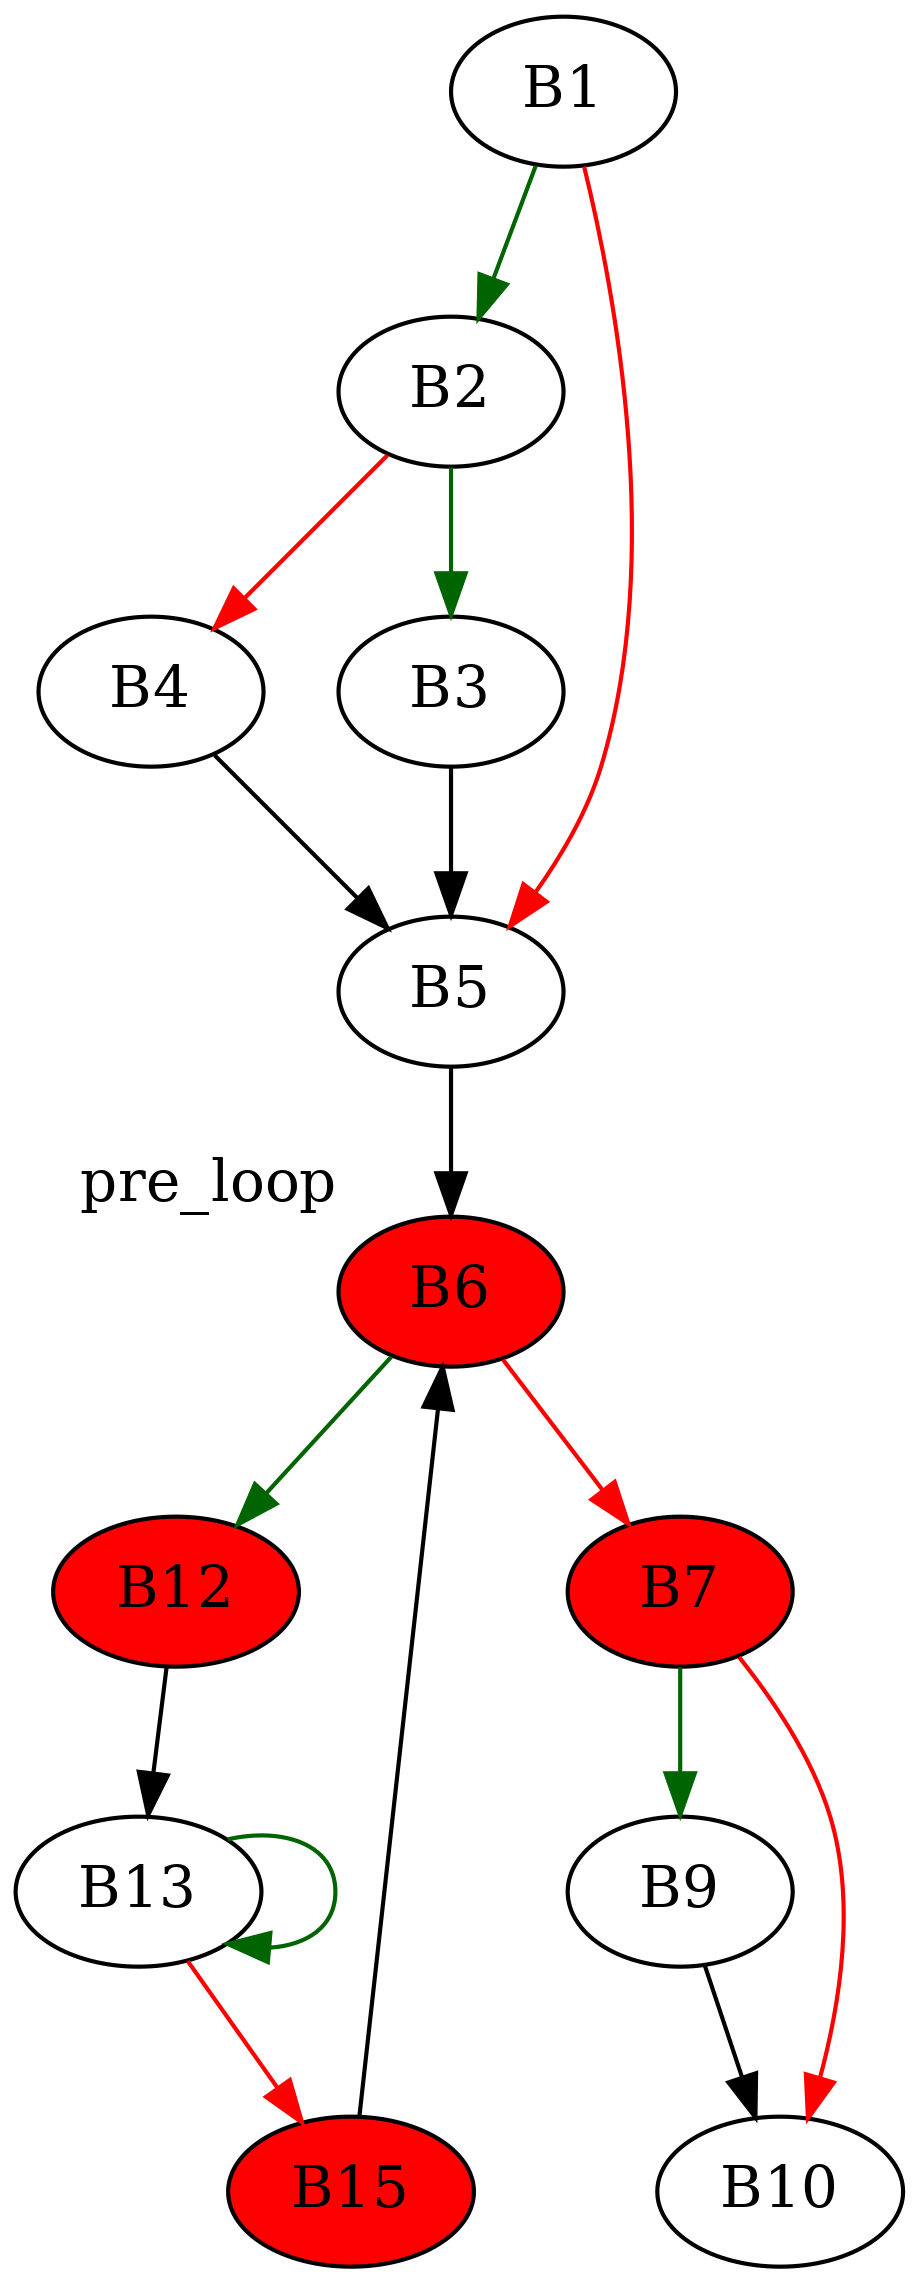
\includegraphics[width=0.6\textwidth]{inc/appendices/examples/interval/example/sample/f_0003a.png}
		\caption{Control flow graph.}
	\end{subfigure}
\end{figure}

\begin{figure}[htbp]
	\centering
	\begin{subfigure}[b]{0.30\textwidth}
		\centering
		\lstinputlisting[linerange={17-43}, linebackgroundcolor={\btLstHL{12-13,19-20}}, language=C, style=c, breaklines=false]{inc/appendices/examples/interval/example/sample.c}
		\caption{Original C source code.}
	\end{subfigure}
	\begin{subfigure}[b]{0.50\textwidth}
		\centering
		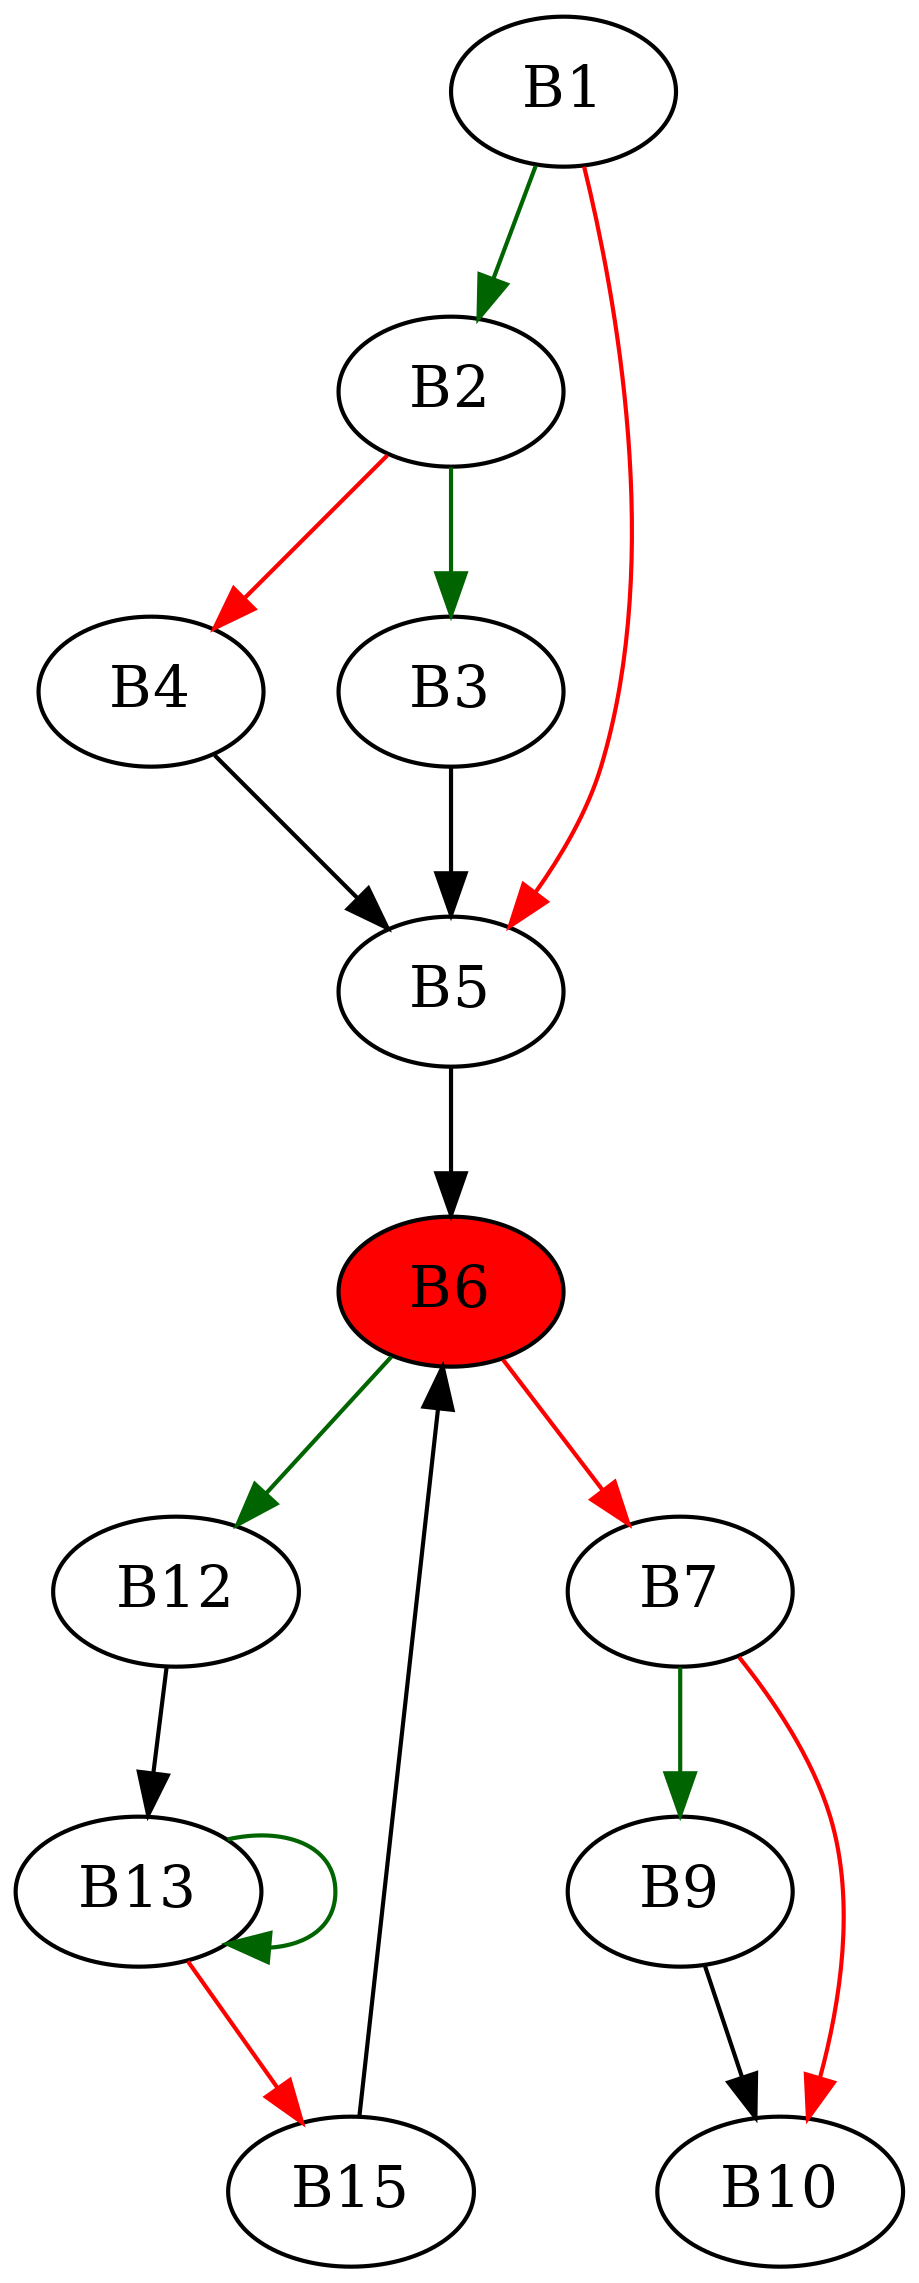
\includegraphics[width=0.6\textwidth]{inc/appendices/examples/interval/example/sample/f_0003b.png}
		\caption{Control flow graph.}
	\end{subfigure}
\end{figure}

\begin{figure}[htbp]
	\centering
	\begin{subfigure}[b]{0.30\textwidth}
		\centering
		\lstinputlisting[linerange={17-43}, linebackgroundcolor={\btLstHL{22-24}}, language=C, style=c, breaklines=false]{inc/appendices/examples/interval/example/sample.c}
		\caption{Original C source code.}
	\end{subfigure}
	\begin{subfigure}[b]{0.50\textwidth}
		\centering
		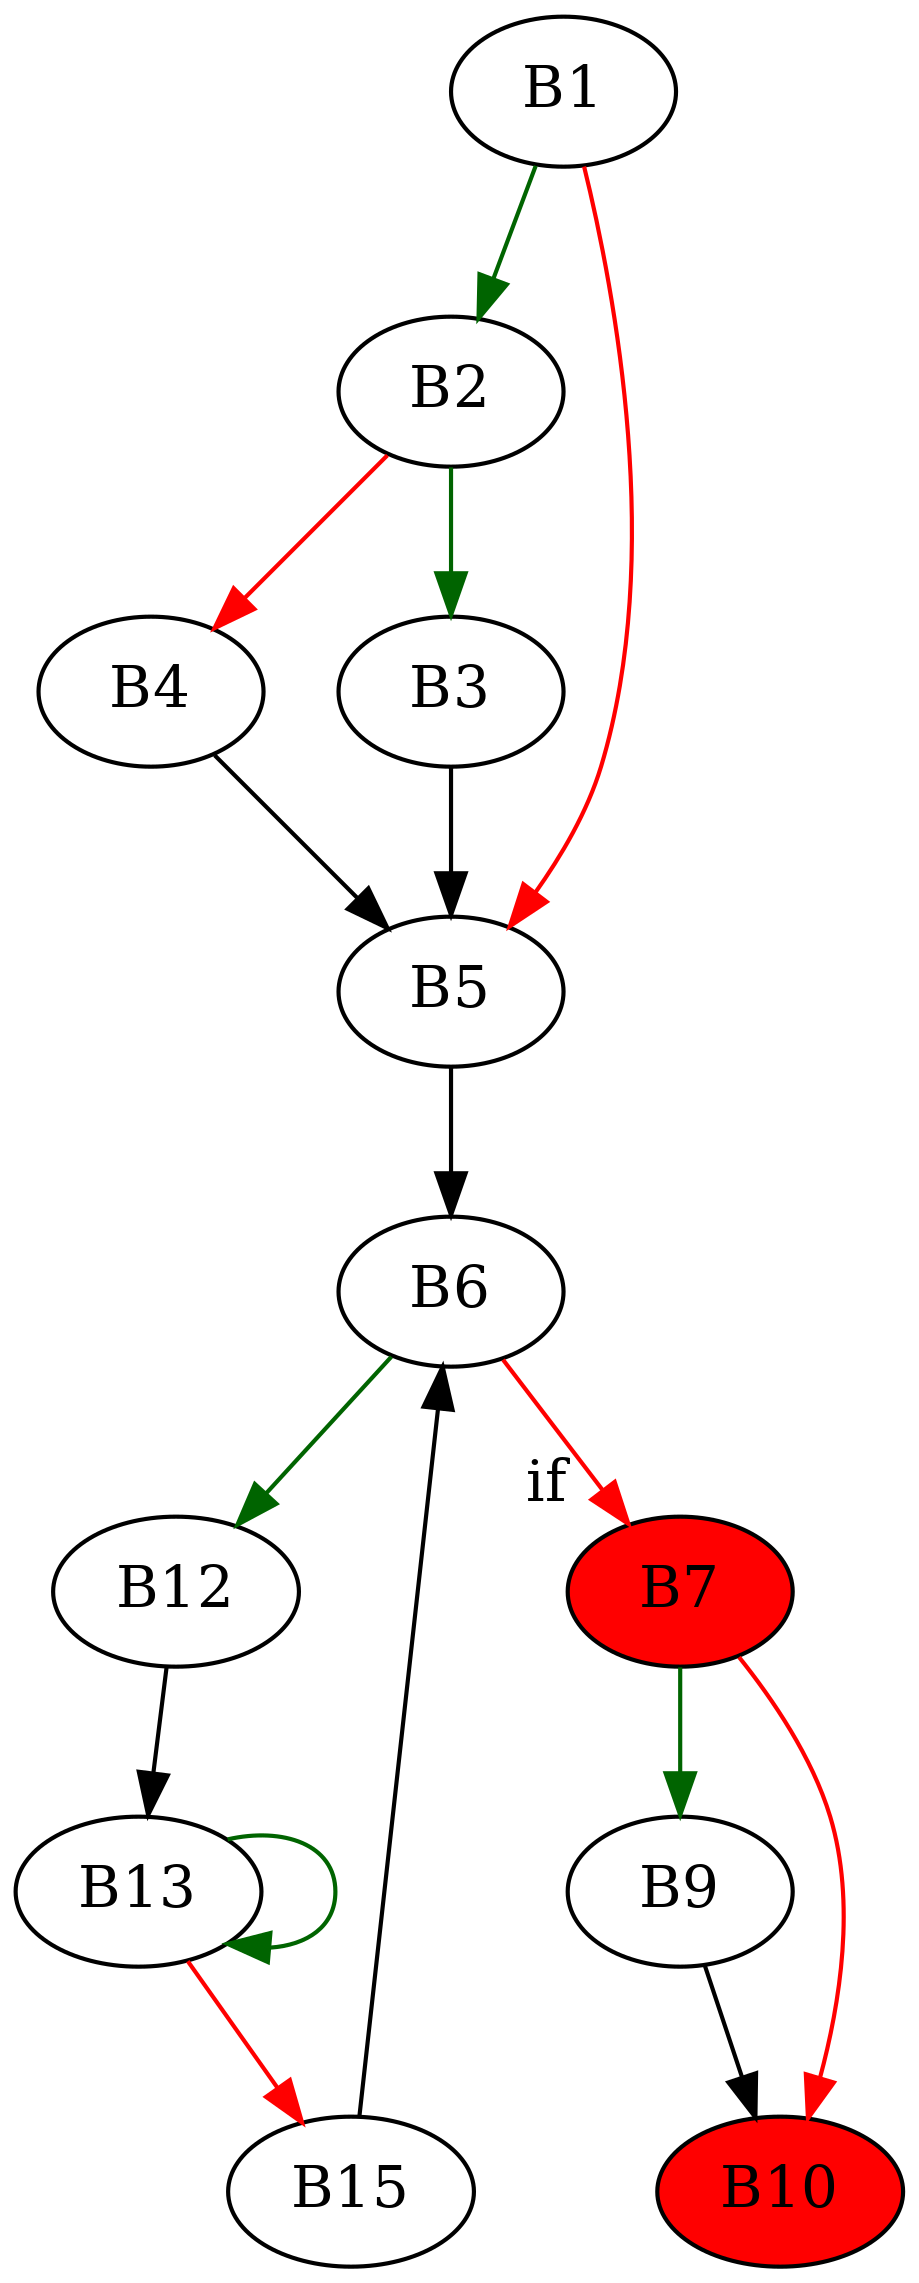
\includegraphics[width=0.6\textwidth]{inc/appendices/examples/interval/example/sample/f_0004a.png}
		\caption{Control flow graph.}
	\end{subfigure}
\end{figure}

\begin{figure}[htbp]
	\centering
	\begin{subfigure}[b]{0.30\textwidth}
		\centering
		\lstinputlisting[linerange={17-43}, linebackgroundcolor={\btLstHL{22-24}}, language=C, style=c, breaklines=false]{inc/appendices/examples/interval/example/sample.c}
		\caption{Original C source code.}
	\end{subfigure}
	\begin{subfigure}[b]{0.50\textwidth}
		\centering
		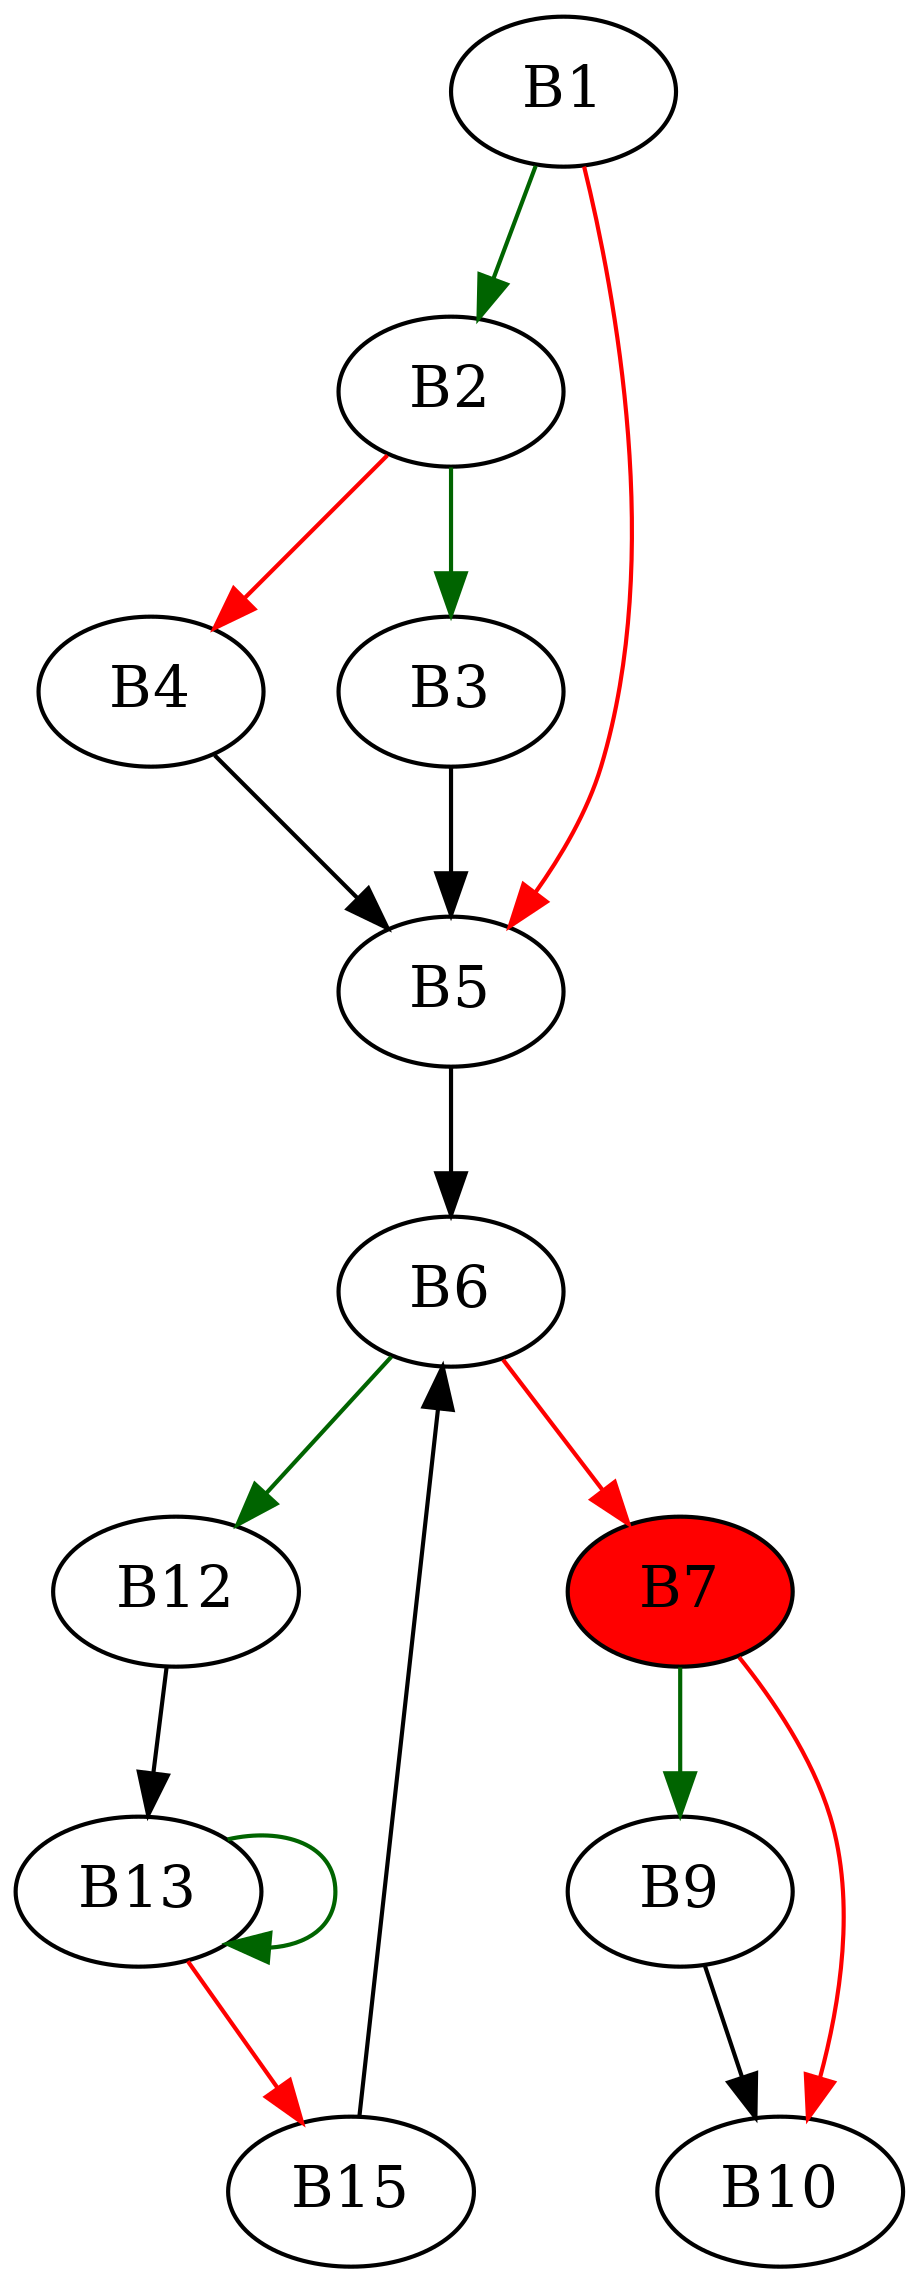
\includegraphics[width=0.6\textwidth]{inc/appendices/examples/interval/example/sample/f_0004b.png}
		\caption{Control flow graph.}
	\end{subfigure}
\end{figure}

\begin{figure}[htbp]
	\centering
	\begin{subfigure}[b]{0.30\textwidth}
		\centering
		\lstinputlisting[linerange={17-43}, linebackgroundcolor={\btLstHL{3,10}}, language=C, style=c, breaklines=false]{inc/appendices/examples/interval/example/sample.c}
		\caption{Original C source code.}
	\end{subfigure}
	\begin{subfigure}[b]{0.50\textwidth}
		\centering
		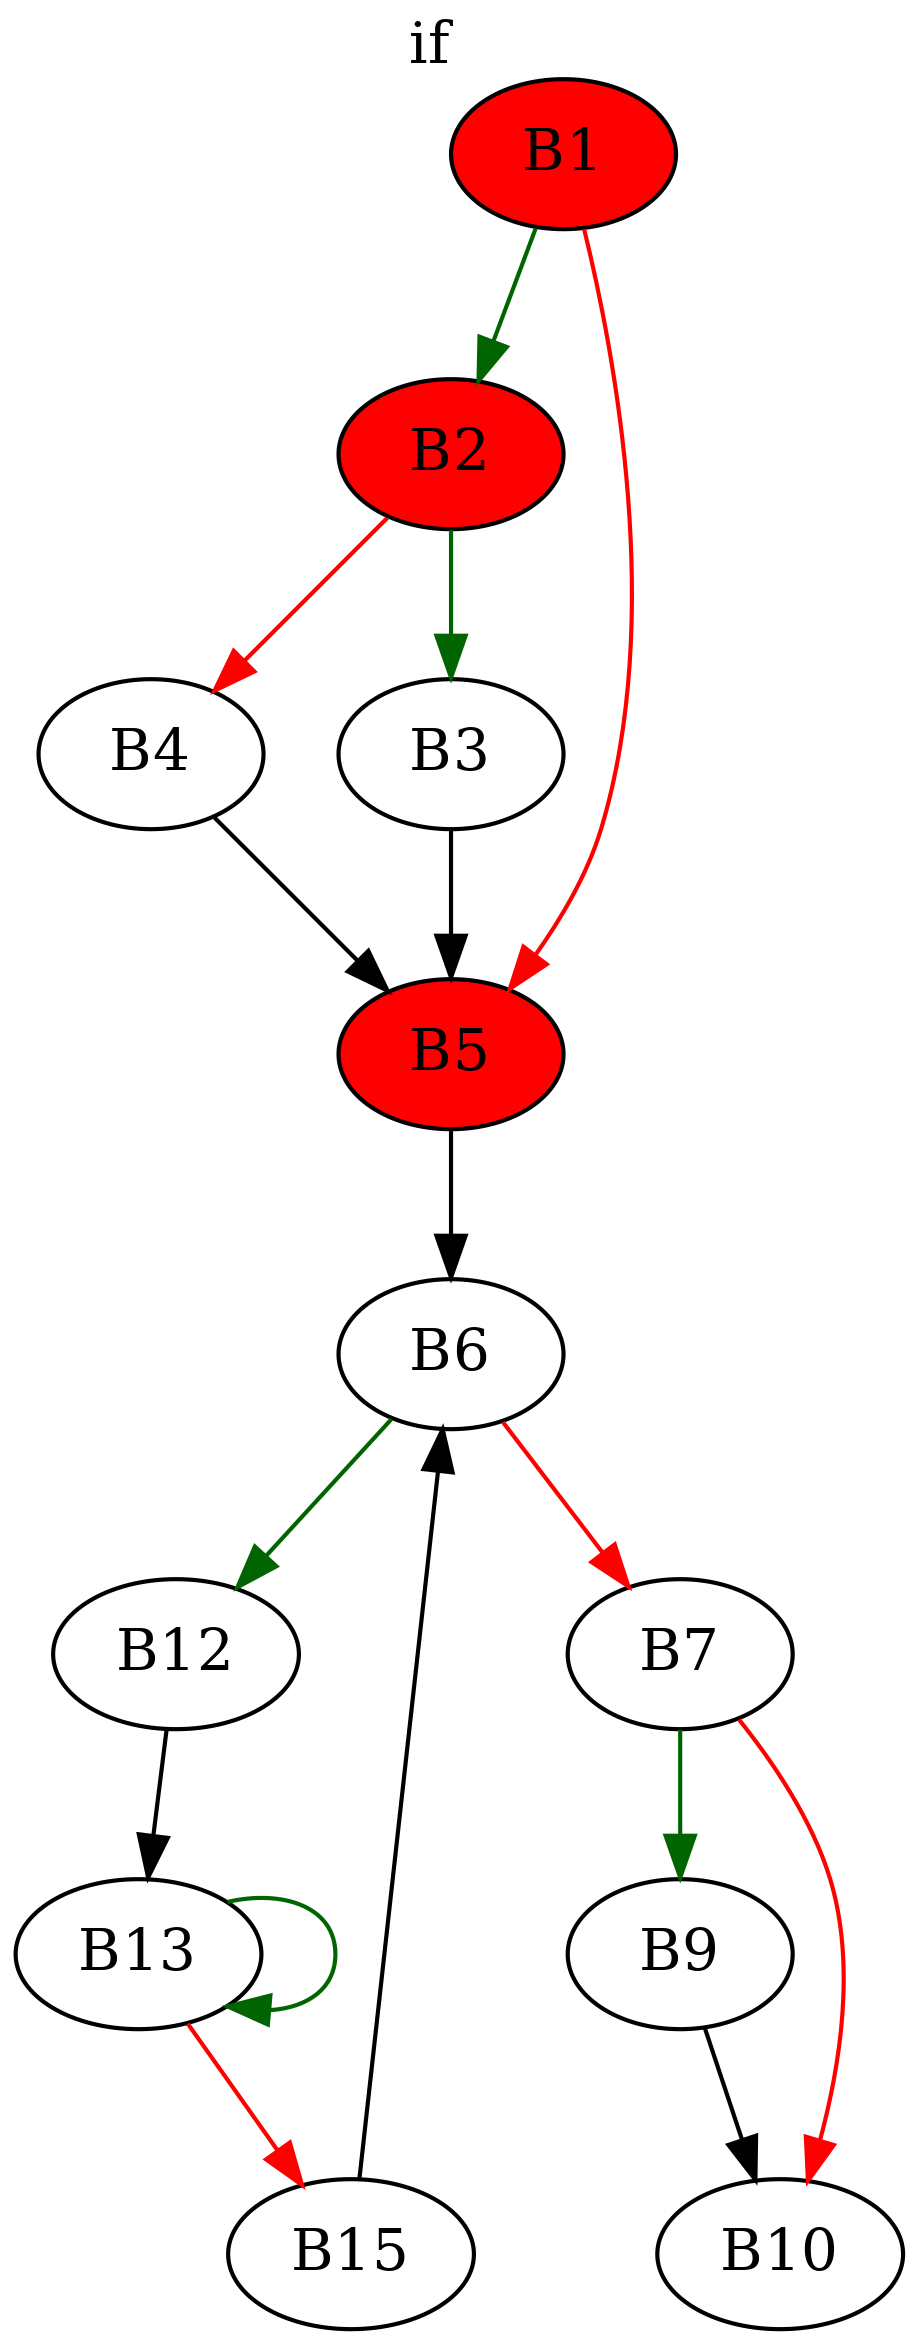
\includegraphics[width=0.6\textwidth]{inc/appendices/examples/interval/example/sample/f_0005a.png}
		\caption{Control flow graph.}
	\end{subfigure}
\end{figure}

\begin{figure}[htbp]
	\centering
	\begin{subfigure}[b]{0.30\textwidth}
		\centering
		\lstinputlisting[linerange={17-43}, linebackgroundcolor={\btLstHL{3,10}}, language=C, style=c, breaklines=false]{inc/appendices/examples/interval/example/sample.c}
		\caption{Original C source code.}
	\end{subfigure}
	\begin{subfigure}[b]{0.50\textwidth}
		\centering
		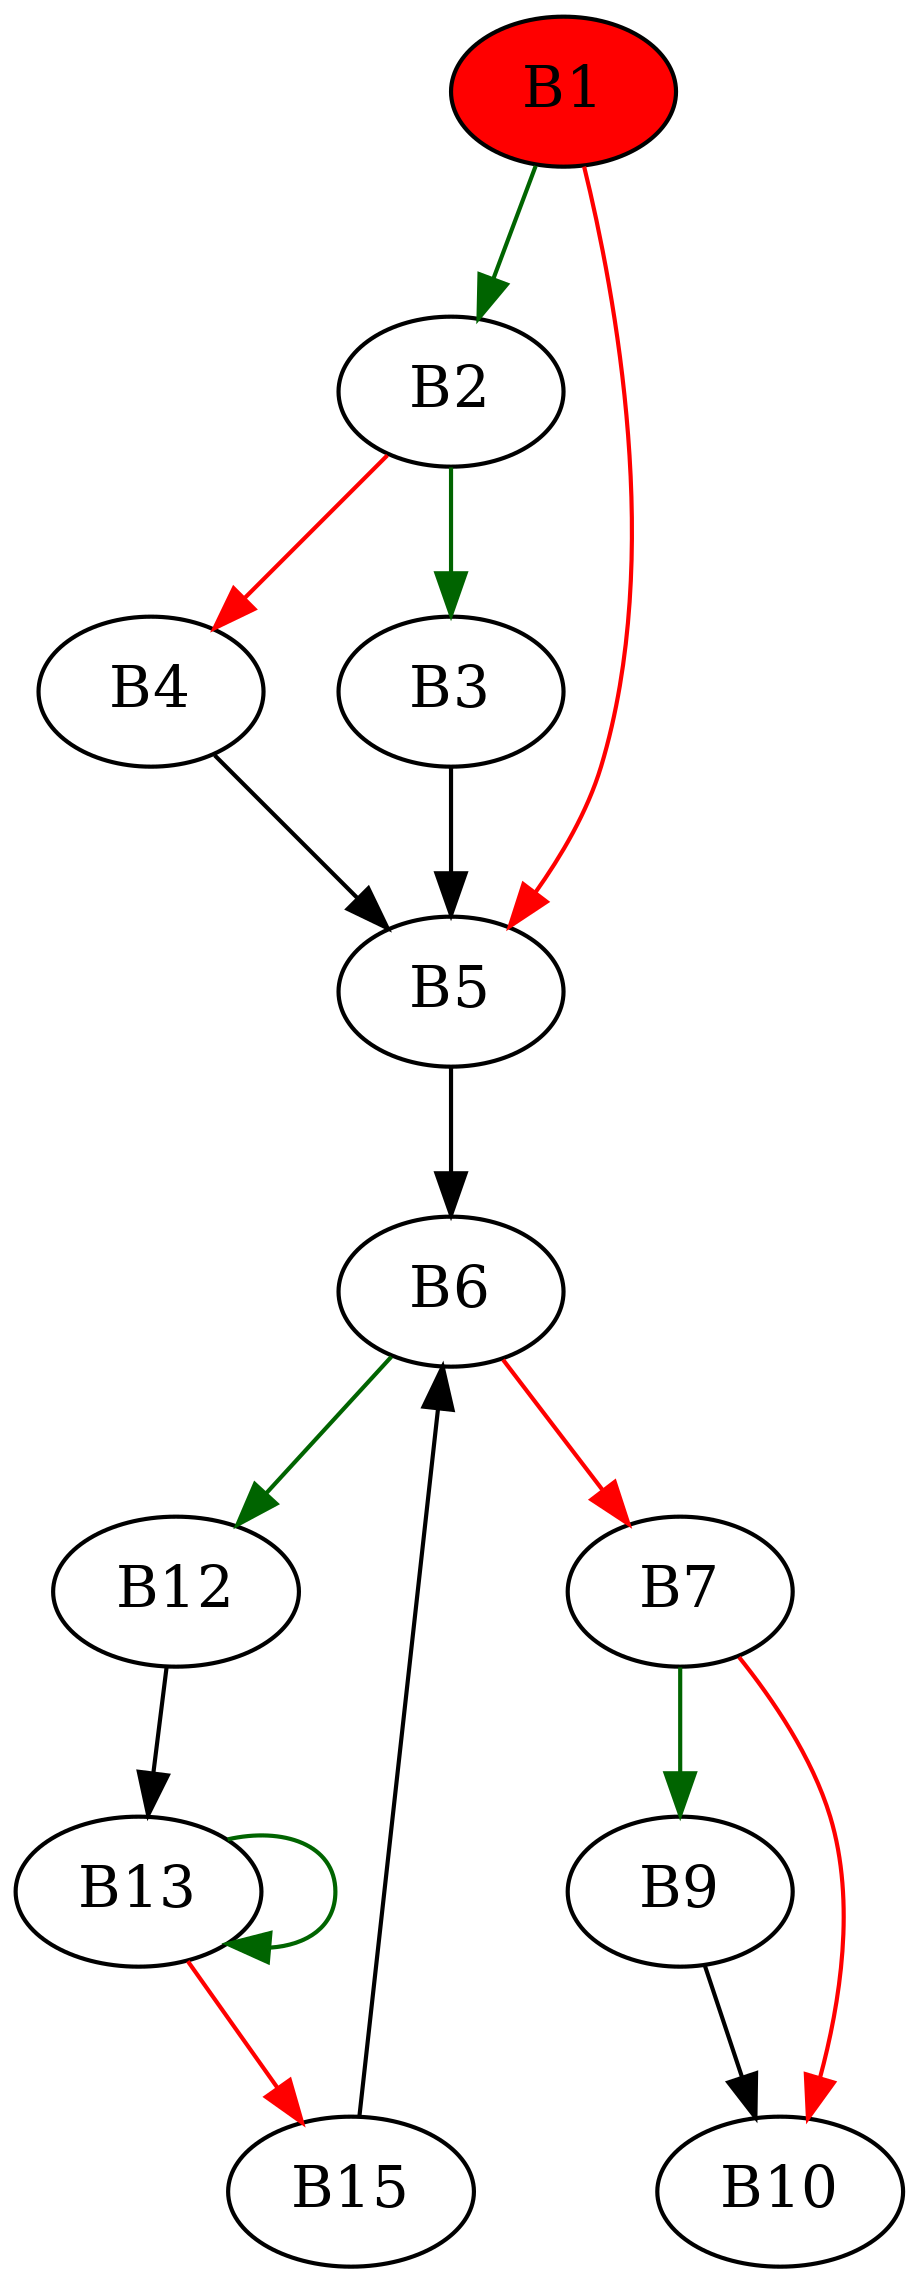
\includegraphics[width=0.6\textwidth]{inc/appendices/examples/interval/example/sample/f_0005b.png}
		\caption{Control flow graph; analysis \textit{almost} \textbf{complete}.}
	\end{subfigure}
\end{figure}

% ___ [ Interval Method - Counter-example 1 ] __________________________________

\clearpage

\subsubsection{Interval Method - Counter-example 1}

Counter-example with \textit{jump threading} optimization and boolean constraint propagation.

\begin{figure}[htbp]
	\centering
	\begin{subfigure}[b]{0.30\textwidth}
		\centering
		\lstinputlisting[linerange={8-21}, language=C, style=c, breaklines=false]{inc/appendices/examples/interval/counter-example/bool_propagation.c}
		\caption{Original C source code.}
	\end{subfigure}
	\begin{subfigure}[b]{0.50\textwidth}
		\centering
		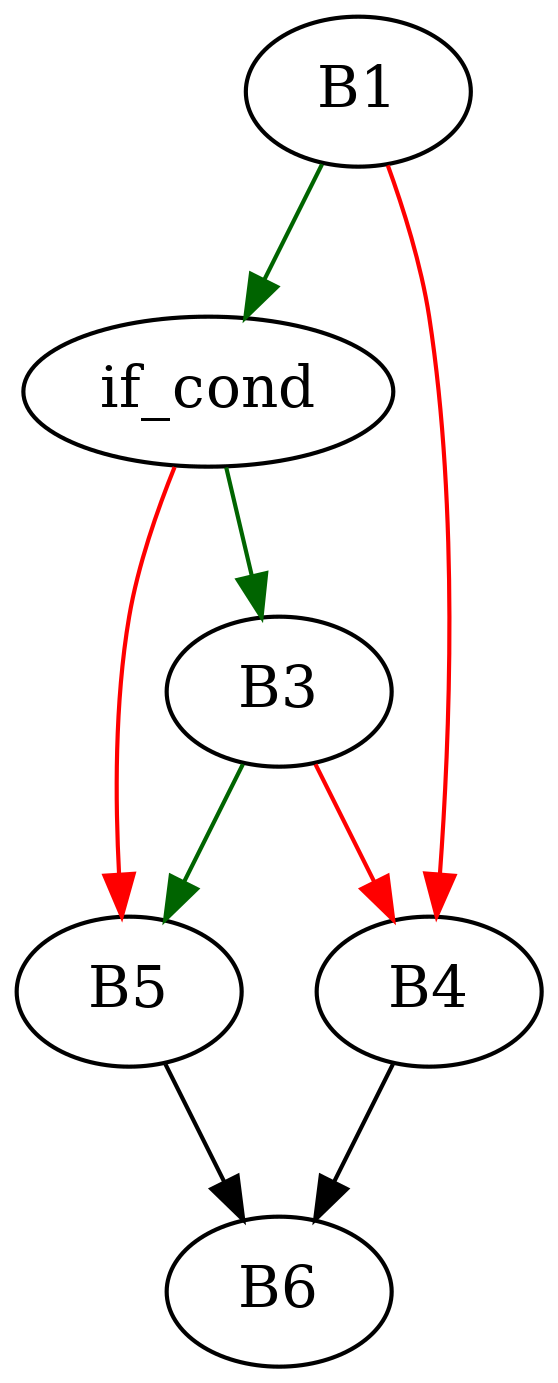
\includegraphics[width=0.35\textwidth]{inc/appendices/examples/interval/counter-example/bool_propagation_jump/f.png}
		\caption{Control flow graph.}
	\end{subfigure}
\end{figure}

\begin{figure}[htbp]
	\centering
	\begin{subfigure}[b]{0.30\textwidth}
		\centering
		\lstinputlisting[linebackgroundcolor={\btLstHL{4-6}}, linerange={8-21}, language=C, style=c, breaklines=false]{inc/appendices/examples/interval/counter-example/bool_propagation.c}
		\caption{Original C source code.}
	\end{subfigure}
	\begin{subfigure}[b]{0.50\textwidth}
		\centering
		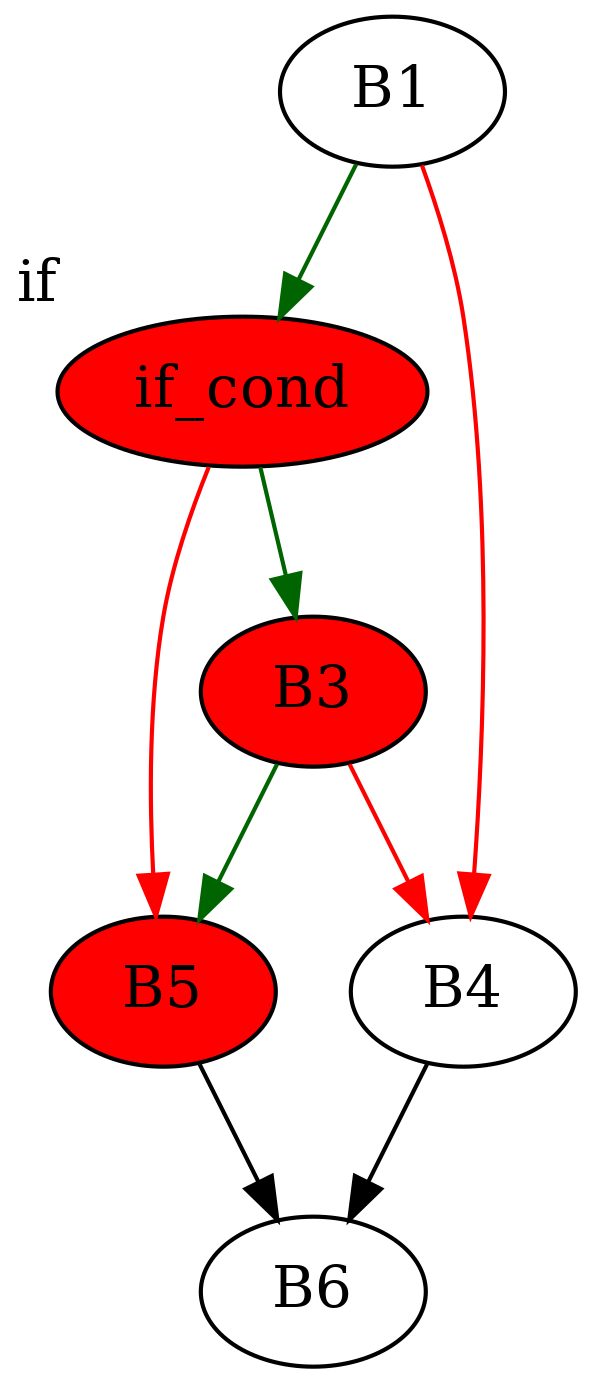
\includegraphics[width=0.35\textwidth]{inc/appendices/examples/interval/counter-example/bool_propagation_jump/f_0001a.png}
		\caption{Control flow graph.}
	\end{subfigure}
\end{figure}

\begin{figure}[htbp]
	\centering
	\begin{subfigure}[b]{0.30\textwidth}
		\centering
		\lstinputlisting[linebackgroundcolor={\btLstHL{4-6}}, linerange={8-21}, language=C, style=c, breaklines=false]{inc/appendices/examples/interval/counter-example/bool_propagation.c}
		\caption{Original C source code.}
	\end{subfigure}
	\begin{subfigure}[b]{0.50\textwidth}
		\centering
		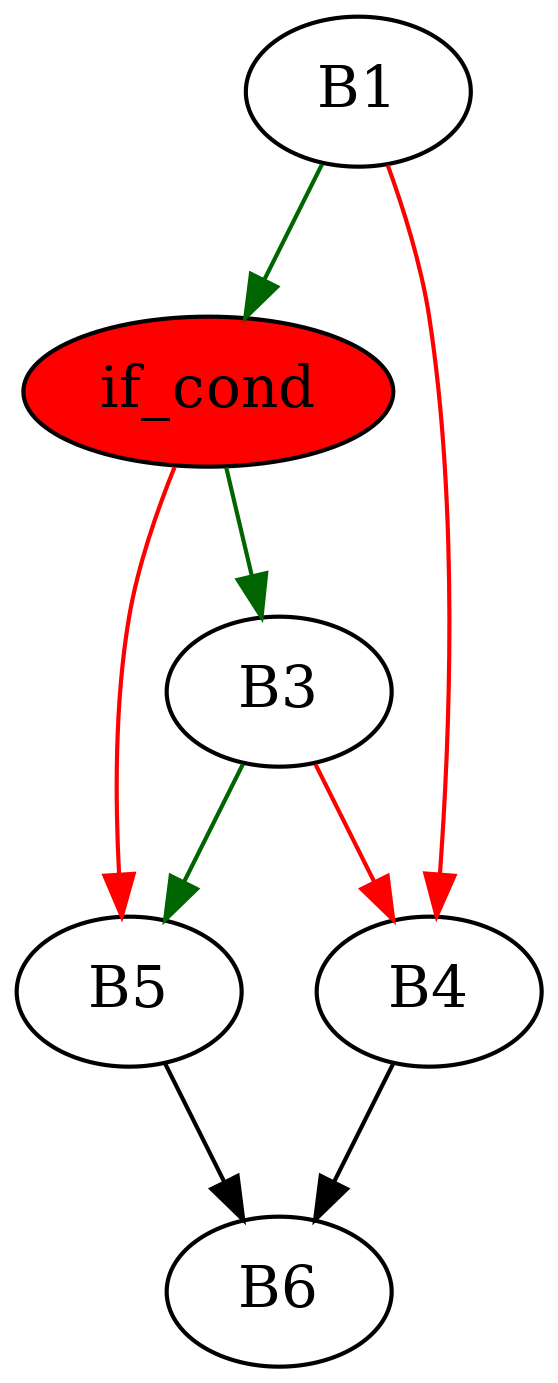
\includegraphics[width=0.35\textwidth]{inc/appendices/examples/interval/counter-example/bool_propagation_jump/f_0001b.png}
		\caption{Control flow graph.}
	\end{subfigure}
\end{figure}

\begin{figure}[htbp]
	\centering
	\begin{subfigure}[b]{0.30\textwidth}
		\centering
		\lstinputlisting[linebackgroundcolor={\btLstHL{4,12}}, linerange={8-21}, language=C, style=c, breaklines=false]{inc/appendices/examples/interval/counter-example/bool_propagation.c}
		\caption{Original C source code.}
	\end{subfigure}
	\begin{subfigure}[b]{0.50\textwidth}
		\centering
		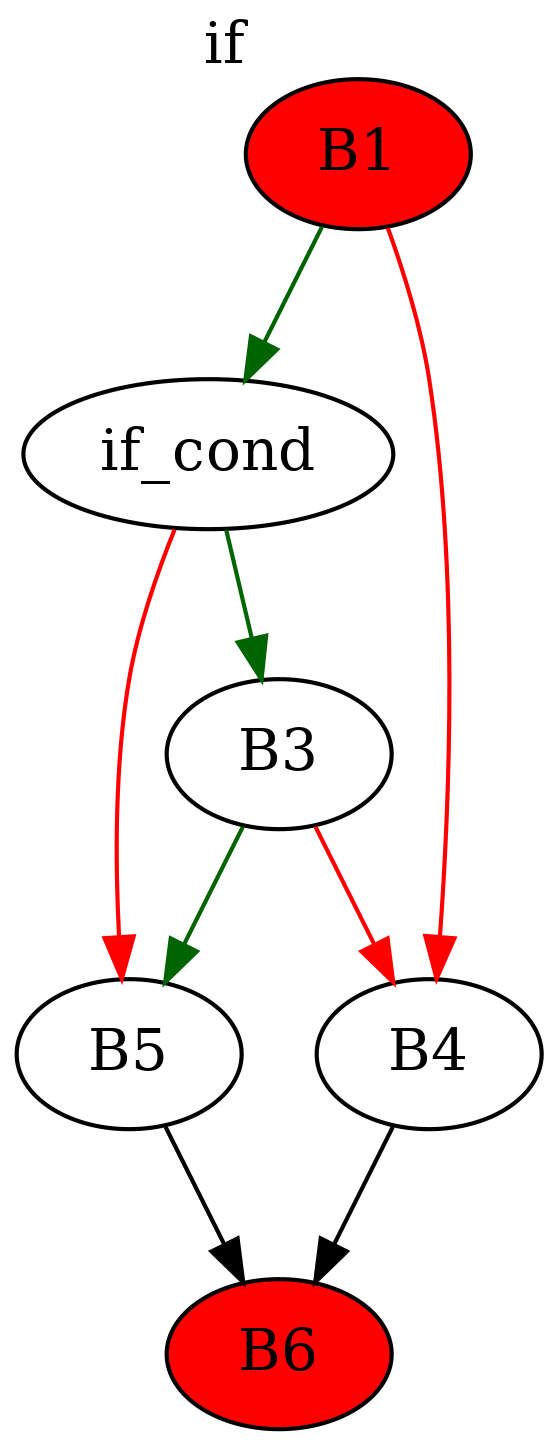
\includegraphics[width=0.35\textwidth]{inc/appendices/examples/interval/counter-example/bool_propagation_jump/f_0002a.png}
		\caption{Control flow graph.}
	\end{subfigure}
\end{figure}

\begin{figure}[htbp]
	\centering
	\begin{subfigure}[b]{0.30\textwidth}
		\centering
		\lstinputlisting[linebackgroundcolor={\btLstHL{4,12}}, linerange={8-21}, language=C, style=c, breaklines=false]{inc/appendices/examples/interval/counter-example/bool_propagation.c}
		\caption{Original C source code.}
	\end{subfigure}
	\begin{subfigure}[b]{0.50\textwidth}
		\centering
		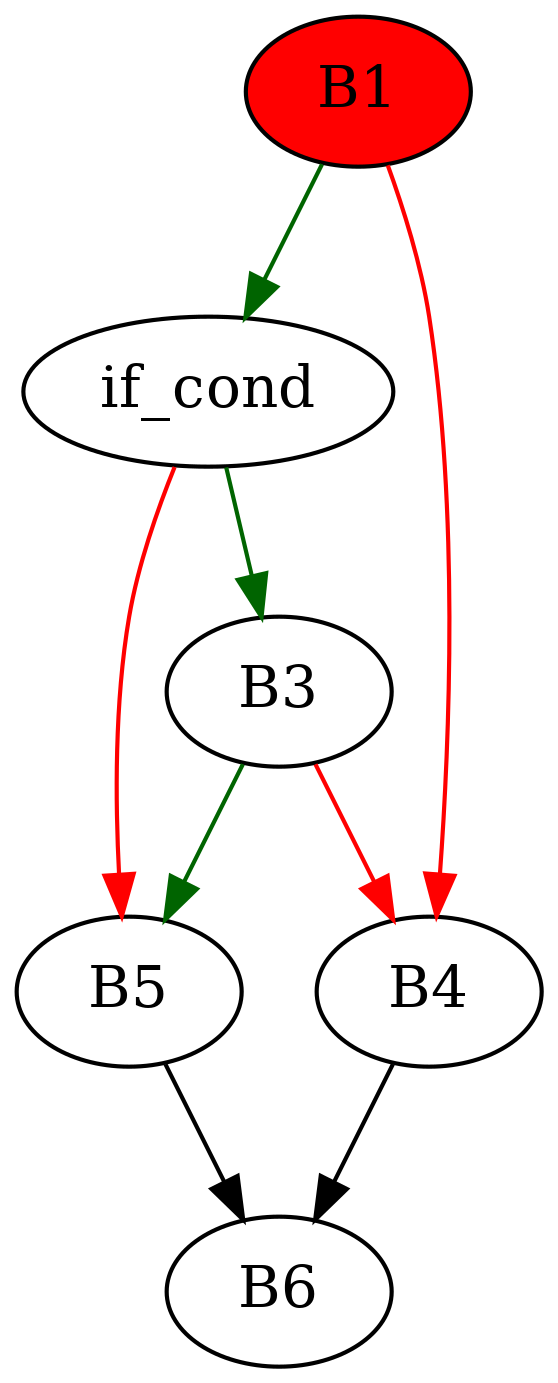
\includegraphics[width=0.35\textwidth]{inc/appendices/examples/interval/counter-example/bool_propagation_jump/f_0002b.png}
		\caption{Control flow graph; analysis \textbf{incomplete}.}
	\end{subfigure}
\end{figure}
